\documentclass[a5paper, 10pt]{article}

% Текст
\usepackage[utf8]{inputenc} % UTF-8 кодировка
\usepackage[russian]{babel} % Русский язык
\usepackage{indentfirst} % красная строка в первом параграфе в главе
% Отображение страниц
\usepackage{geometry} % размеры листа и отступов
\usepackage{listings}
\usepackage{color}
\usepackage{array}
\usepackage{tabularx}
\renewcommand{\arraystretch}{2} % увеличивает высоту строк в 2 раза
\usepackage{float}
\floatplacement{figure}{H}

\geometry{
	left=12mm,
	top=25mm,
	right=15mm,
	bottom=17mm,
	marginparsep=0mm,
	marginparwidth=0mm,
	headheight=10mm,
	headsep=7mm,
	nofoot}
\usepackage{afterpage,fancyhdr} % настройка колонтитулов
\pagestyle{fancy}
\fancypagestyle{style}{ % создание нового стиля style
	\fancyhf{} % очистка колонтитулов
	\fancyhead[LO, RE]{ЛР № 4 } % название документа наверху
	\fancyhead[RO, LE]{Точностные свойства системы, астатизмы и регуляторы} % название section наверху
	\fancyfoot[RO, LE]{\thepage} % номер страницы справа внизу на нечетных и слева внизу на четных
	\renewcommand{\headrulewidth}{0.25pt} % толщина линии сверху
	\renewcommand{\footrulewidth}{0pt} % толцина линии снизу
}
\fancypagestyle{plain}{ % создание нового стиля plain -- полностью пустого
	\fancyhf{}
	\renewcommand{\headrulewidth}{0pt}
}
\fancypagestyle{title}{ % создание нового стиля title -- для титульной страницы
	\fancyhf{}
	\fancyhead[C]{{\footnotesize
			Министерство образования и науки Российской Федерации\\
			Федеральное государственное автономное образовательное учреждение высшего образования
	}}
	\fancyfoot[C]{{\large 
			Санкт-Петербург, 2026
	}}
	\renewcommand{\headrulewidth}{0pt}
}

%Программирование
\usepackage{listings}

\definecolor{codegreen}{rgb}{0,0.6,0}
\definecolor{codegray}{rgb}{0.5,0.5,0.5}
\definecolor{codepurple}{rgb}{0.58,0,0.82}
\definecolor{backcolour}{rgb}{0.95,0.95,0.92}

\lstdefinestyle{codestyle}{
    backgroundcolor=\color{backcolour},
    keywordstyle=\color{magenta},
    numberstyle=\tiny\color{codegray},
    stringstyle=\color{codepurple},
    basicstyle=\ttfamily\footnotesize,
    breakatwhitespace=false,
    breaklines=true,
    captionpos=b,
    keepspaces=true,
    numbers=left,
    numbersep=5pt,
    showspaces=false,
    showstringspaces=false, % показывать или нет пробелы специальными отступами
    showtabs=false, % показывать или нет табуляцию в строках
    tabsize=2 % размер табуляции по умолчанию равен 2 пробелам
}
\lstset{
    language=Python, % Язык программирования
    basicstyle=\ttfamily\small, % Стиль текста
    commentstyle=\color{green}, % Стиль комментариев
    keywordstyle=\color{blue}, % Стиль ключевых слов
    stringstyle=\color{red}, % Стиль строк
    showstringspaces=false, % Не показывать пробелы в строках
    breaklines=true, % Переносить длинные строки
    extendedchars=true, % Поддержка кириллицы
    inputencoding=utf8, % Кодировка входного файла
    numbers=left,               % где поставить нумерацию строк (слева\справа)
    numberstyle=\tiny,           % размер шрифта для номеров строк
    stepnumber=1,                   % размер шага между двумя номерами строк
    numbersep=5pt,                % как далеко отстоят номера строк от подсвечиваемого кода
    captionpos=b,              % позиция заголовка вверху [t] или внизу [b] 
    breaklines=true,           % автоматически переносить строки (да\нет)
    breakatwhitespace=false, % переносить строки только если есть пробел
    literate={а}{{\cyra}}1 {б}{{\cyrb}}1 {в}{{\cyrv}}1 {г}{{\cyrg}}1 {д}{{\cyrd}}1
             {е}{{\cyre}}1 {ё}{{\cyryo}}1 {ж}{{\cyrzh}}1 {з}{{\cyrz}}1 {и}{{\cyri}}1
             {й}{{\cyrishrt}}1 {к}{{\cyrk}}1 {л}{{\cyrl}}1 {м}{{\cyrm}}1 {н}{{\cyrn}}1
             {о}{{\cyro}}1 {п}{{\cyrp}}1 {р}{{\cyrr}}1 {с}{{\cyrs}}1 {т}{{\cyrt}}1
             {у}{{\cyru}}1 {ф}{{\cyrf}}1 {х}{{\cyrh}}1 {ц}{{\cyrc}}1 {ч}{{\cyrch}}1
             {ш}{{\cyrsh}}1 {щ}{{\cyrshch}}1 {ъ}{{\cyrhrdsn}}1 {ы}{{\cyrery}}1
             {ь}{{\cyrsftsn}}1 {э}{{\cyrerev}}1 {ю}{{\cyryu}}1 {я}{{\cyrya}}1
             {А}{{\CYRA}}1 {Б}{{\CYRB}}1 {В}{{\CYRV}}1 {Г}{{\CYRG}}1 {Д}{{\CYRD}}1
             {Е}{{\CYRE}}1 {Ё}{{\CYRYO}}1 {Ж}{{\CYRZH}}1 {З}{{\CYRZ}}1 {И}{{\CYRI}}1
             {Й}{{\CYRISHRT}}1 {К}{{\CYRK}}1 {Л}{{\CYRL}}1 {М}{{\CYRM}}1 {Н}{{\CYRN}}1
             {О}{{\CYRO}}1 {П}{{\CYRP}}1 {Р}{{\CYRR}}1 {С}{{\CYRS}}1 {Т}{{\CYRT}}1
             {У}{{\CYRU}}1 {Ф}{{\CYRF}}1 {Х}{{\CYRH}}1 {Ц}{{\CYRC}}1 {Ч}{{\CYRCH}}1
             {Ш}{{\CYRSH}}1 {Щ}{{\CYRSHCH}}1 {Ъ}{{\CYRHRDSN}}1 {Ы}{{\CYRERY}}1
             {Ь}{{\CYRSFTSN}}1 {Э}{{\CYREREV}}1 {Ю}{{\CYRYU}}1 {Я}{{\CYRYA}}1,
}

\lstset{style=codestyle}

% Математика
\usepackage{amsmath, amsfonts, amssymb, amsthm} % Набор пакетов для математических текстов
%\usepackage{dmvnbase} % мехматовский пакет latex-сокращений
\usepackage{cancel} % зачеркивание для сокращений
% Рисунки и фигуры
\usepackage[pdftex]{graphicx} % вставка рисунков
\usepackage{wrapfig, subcaption} % вставка фигур, обтекая текст
\usepackage{caption} % для настройки подписей
\captionsetup{figurewithin=none,labelsep=period, font={small,it}} % настройка подписей к рисункам
% Рисование
\usepackage{tikz} % рисование
\usepackage{circuitikz}
\usepackage{pgfplots} % графики
% Таблицы
\usepackage{multirow} % объединение строк
\usepackage{multicol} % объединение столбцов
% Остальное
%\usepackage[unicode, pdftex]{hyperref} % гиперссылки
\usepackage[colorlinks]{hyperref} % гиперссылки
\hypersetup{
    linkcolor=blue,
    filecolor=magenta,
    urlcolor=cyan
}
\usepackage{enumitem} % нормальное оформление списков
\setlist{itemsep=0.15cm,topsep=0.15cm,parsep=1pt} % настройки списков
% Теоремы, леммы, определения...
\theoremstyle{definition}
\newtheorem{Def}{Определение}
\newtheorem*{Axiom}{Аксиома}
\theoremstyle{plain}
\newtheorem{Th}{Теорема}
\newtheorem{Lem}{Лемма}
\newtheorem{Cor}{Следствие}
\newtheorem{Ex}{Пример}
\theoremstyle{remark}
\newtheorem*{Note}{Замечание}
\newtheorem*{Solution}{Решение}
\newtheorem*{Proof}{Доказательство}
% Свои команды
\newcommand{\comb}[1]{\left[\hspace{-4pt}\begin{array}{l}#1\end{array}\right.\hspace{-5pt} } % совокупность уравнений
% Титульный лист
\usepackage{csvsimple-l3}
\newcommand*{\titlePage}{
	\thispagestyle{title}
	\begingroup
	\begin{center}
		%		{\footnotesize
			%			Министерство образования и науки Российской Федерации\\
			%			Федеральное государственное автономное образовательное учреждение высшего образования
			%		}
		%		
		\vspace*{6ex}
		
		{\small
			САНКТ-ПЕТЕРБУРГСКИЙ НАЦИОНАЛЬНЫЙ ИССЛЕДОВАТЕЛЬСКИЙ УНИВЕРСИТЕТ ИТМО	
		}
		
		\vspace*{2ex}
		
		{\normalsize
			Факультет систем управления и робототехники
		}
		
		\vspace*{15ex}
		
		{\Large \bfseries 
			Лабораторная работа № 4
		}
\vspace*{2ex}
	{\Large \bfseries 
			
<<Точностные свойства системы, астатизмы и регуляторы>>
		}
\vspace*{2ex}
		
		{\normalsize
			по дисциплине ЛСАУ
		}
\vspace*{2ex}
	{\Large \bfseries 
			
Вариант 30
		}

	\end{center}
	\vspace*{8ex}
	\begin{flushright}
		{\large 
			\underline{Выполнил}:\\
			\begin{flushright}
				студент гр. \textbf{R3380} \textbf{Янушанец Р. Д.}\\
			\end{flushright}
		}
		
		\vspace*{6ex}
		
		{\large 
			\underline{Преподаватель}:\\
            \begin{flushright}
            \textbf{Пашенко Артём Витальевич}
            \end{flushright}
		}
	\end{flushright}
	\newpage
	\setcounter{page}{1}
	\endgroup}

\begin{document}
	\titlePage
	\pagestyle{style}
\newpage

\tableofcontents

\newpage

\section{Задание 1. Задача стабилизации с "идеальным" дифференцирующим звеном}

\subsection{Исходные данные}
Объект управления описывается дифференциальным уравнением:
\begin{equation} \label{eq:object}
a_2\ddot{y} + a_1\dot{y} + a_0y = u
\end{equation}

Рассмотрим регулятор вида:

\begin{equation} \label{eq:regulator}
    u = k_0 y + k_1 \dot{y}
    \end{equation}


\subsection{Аналитические расчеты}

Найдем передаточную функцию нашего объекта:

$$
W(s)=\dfrac{1}{a_2s^2+a_1s+a_0}
$$

$$
W(s)=\dfrac{\dfrac{1}{a_2}}{s^2+\dfrac{a_1}{a_2}s+\dfrac{a_0}{a_2}}
$$

Корни характеристического уравнения будут находится следующим образом:

$$
\lambda=\dfrac{-\dfrac{a_1}{a_2}\pm\sqrt{\left(\dfrac{a_1}{a_2}\right)^2-4\dfrac{a_0}{a_2}}}{2}
$$

Возьмём коэффициенты равные:

$$
a_2=1 \qquad a_1 = - 6 \qquad a_0 = -7 
$$

Тогда корни характеристического уровнения будут равны:

$$
\lambda_1=7 \ - \ \textbf{неустойчивый} \qquad \lambda_2=-1 \ - \ \textbf{устойчивый}
$$

Подставим регулятор:

$$
\ddot{y} - 6\dot{y} - 7y = k_0 y + k_1 \dot{y}
$$

$$
\ddot{y}+\dot{y}(-6-k_1)+y(-7-k_0)=0
$$

Для устойчивости замкнутой системы нам необходимо выполнение критериев Гурвинца:

$$
\begin{cases}
    -6-k_1>0\\
    -7-k_0>0
\end{cases}
$$

Пусть коэффициенты будут равны:

$$
k_1=-7 \qquad k_0=-8
$$

Возьмем начальные условия равные:

$$
y(0)=0 \qquad \dot{y}(0)=2
$$

\subsection{Структурные схемы}

\begin{figure}
    \centering
    \includegraphics[width=1\linewidth]{images/image_4_1_1.png}
    \caption{Структурная схема разомкнутой системы}
    \label{fig:placeholder}
\end{figure}

\begin{figure}
    \centering
    \includegraphics[width=1\linewidth]{images/image_4_1_2.png}
    \caption{Структурная схема замкнутой системы}
    \label{fig:placeholder}
\end{figure}

\subsection{Графики выходов}

\begin{figure}[H]
    \centering
    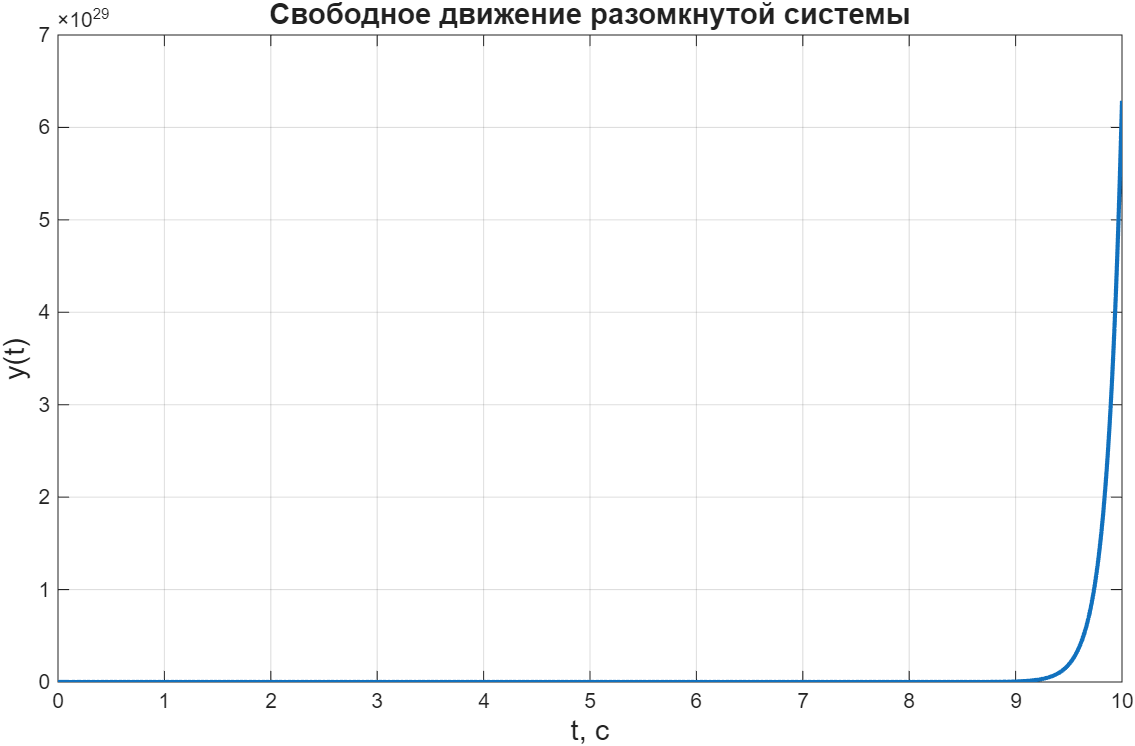
\includegraphics[width=1\linewidth]{images/Figure_4_1_1.png}
    \caption{График свободного движения размокнутой системы}
    \label{fig:placeholder}
\end{figure}

\begin{figure}[H]
    \centering
    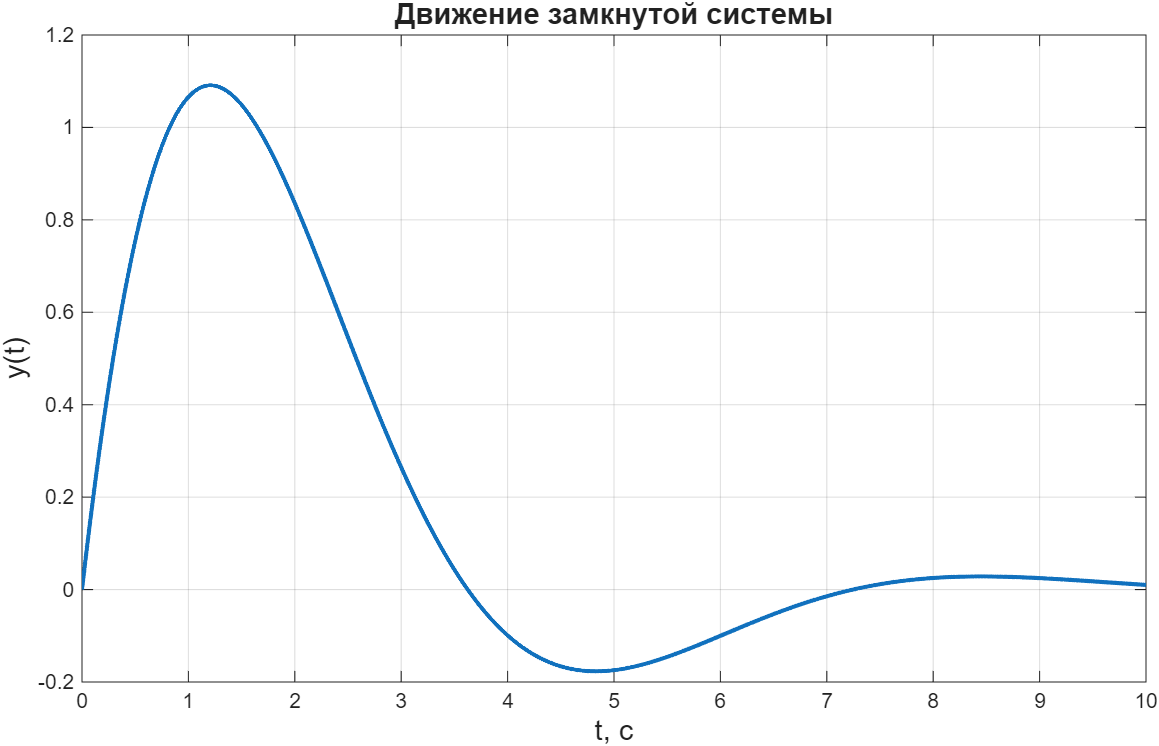
\includegraphics[width=1\linewidth]{images/Figure_4_1_2.png}
    \caption{График выхода замкнутой системы}
    \label{fig:placeholder}
\end{figure}

\subsection{Выводы}

В рамках первого задания был рассмотрен объект второго порядка, содержащий неустойчивый полюс.

Для стабилизации объекта был введён регулятор вида
\[
u = k_0 y + k_1 \dot{y},
\]
содержащий "идеальное" дифференцирующее звено реализованное с помощью блока Derivative. Аналитически, с использованием критерия Гурвица, были определены условия на параметры $k_0$ и $k_1$, при которых замкнутая система является асимптотически устойчивой. Были выбраны конкретные значения коэффициентов, удовлетворяющие найденным условиям устойчивости.

Таким образом, введение "идеального" дифференцирующего звена позволило компенсировать неустойчивость исходного объекта и обеспечить асимптотическую устойчивость замкнутой системы. 


\newpage

\section{Задание 2. Задача стабилизации с реальным дифференцирующим звеном}

\subsection{Исходные данные}

Заменим аппроксимацию производной $\dot{y}$ на передаточную функцию вида:

$$
W_\text{р.дифф.}(p)=\dfrac{p}{Tp+1}
$$

\subsection{Аналитические расчеты}

Подставим регулятор в уравнение объекта:

$$
(s^2-6s-7)Y(s)=-8Y(s)-7\cdot \dfrac{s}{Ts+1}Y(s)
$$

Домножим на $Ts+1$:

$$
(Ts+1)(s^2-6s-7)+(Ts+1)8+7s=0
$$

$$
s^3T+s^2(1-6T)+s(T+1)+1=0
$$

$$
s^3+s^2\dfrac{1-6T}{T}+s\dfrac{T+1}{T}+\dfrac{1}{T}=0
$$

Используя критерий Гурвинца находим $T$ при коорых система асимптотически устойчива:

$$
\begin{cases}
    \dfrac{1}{T}>0\\\\
    \dfrac{T+1}{T}>0\\\\
    \dfrac{1-6T}{T}>0\\\\
    \dfrac{T+2}{T}\cdot\dfrac{1-6T}{T}>\dfrac{1}{T}
\end{cases}
$$
\vspace{0.3cm}

$$
\begin{cases}
    T>0\\\\
    T \in (-\infty,-1)\cup(0,\infty)\\\\
    T \in \left(0,\dfrac{1}{6}\right)\\\\
    T \in \left(\dfrac{-3-\sqrt{15}}{6},\dfrac{-3+\sqrt{15}}{6}\right)
\end{cases}
$$

Таким образом диапазон значений T, при которых система будет асимптотически устойчива:

$$
T\in \left(0, 0.1455 \right)
$$

\subsection{Структурные схемы}

\begin{figure}[H]
    \centering
    \includegraphics[width=0.8\linewidth]{images/image_4_2_1.png}
    \caption{Структурная схема с реальным дифференцирующим звеном}
    \label{fig:placeholder}
\end{figure}

\subsection{Графики выходов}

\begin{figure}[H]
    \centering
    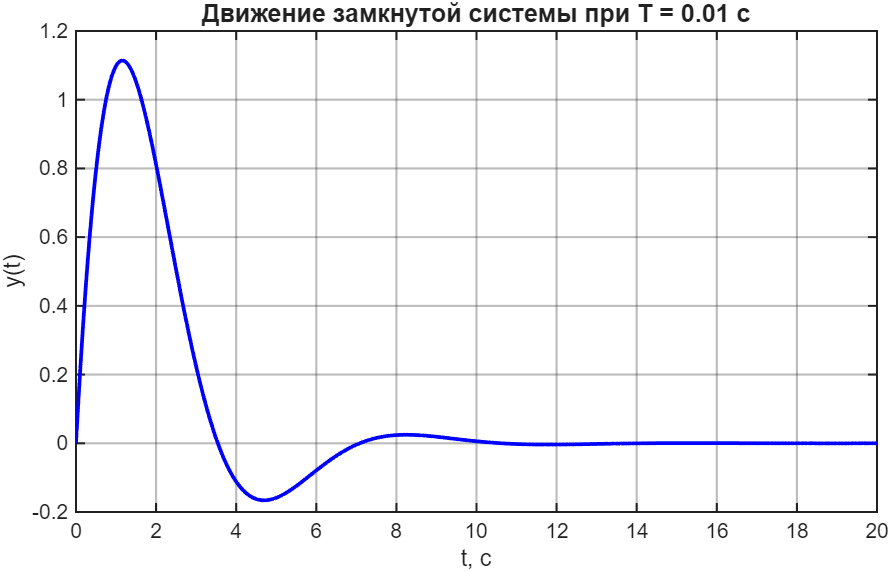
\includegraphics[width=0.8\linewidth]{images/Figure_4_2_1.png}
    \caption{График движения замкнутой системы при $T=0.01$}
    \label{fig:placeholder}
\end{figure}

\begin{figure}[H]
    \centering
    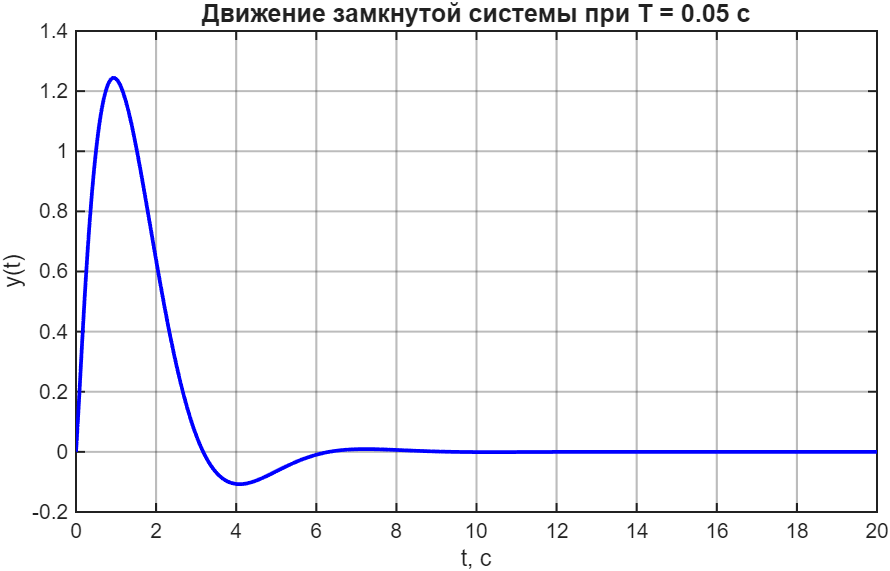
\includegraphics[width=0.8\linewidth]{images/Figure_4_2_2.png}
    \caption{График движения замкнутой системы при $T=0.05$}
    \label{fig:placeholder}
\end{figure}

\begin{figure}[H]
    \centering
    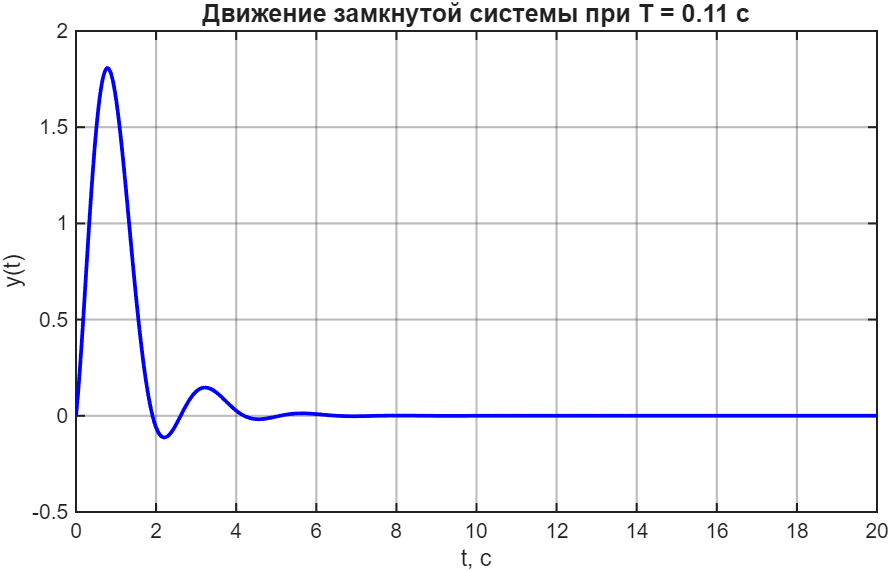
\includegraphics[width=0.8\linewidth]{images/Figure_4_2_3.png}
    \caption{График движения замкнутой системы при $T=0.11$}
    \label{fig:placeholder}
\end{figure}

\begin{figure}[H]
    \centering
    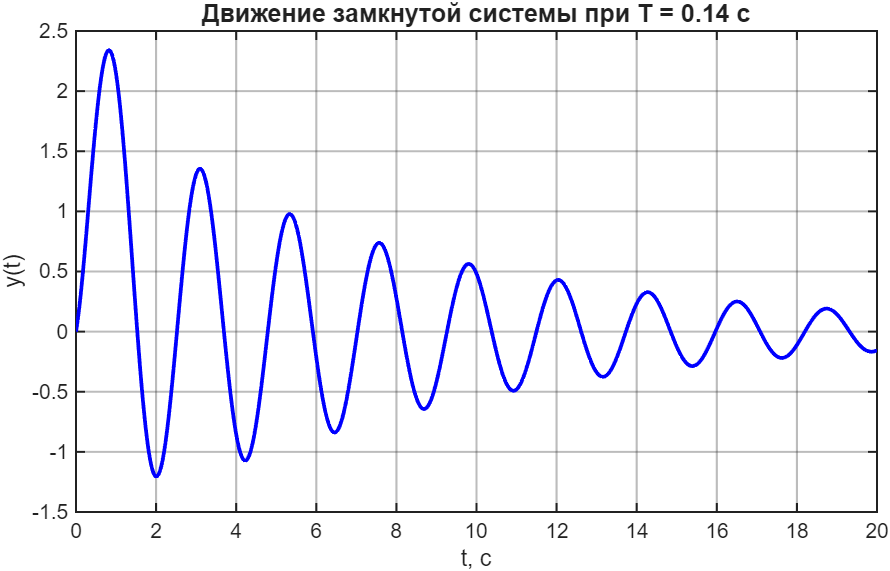
\includegraphics[width=0.8\linewidth]{images/Figure_4_2_4.png}
    \caption{График движения замкнутой системы при $T=0.14$}
    \label{fig:placeholder}
\end{figure}

\begin{figure}[H]
    \centering
    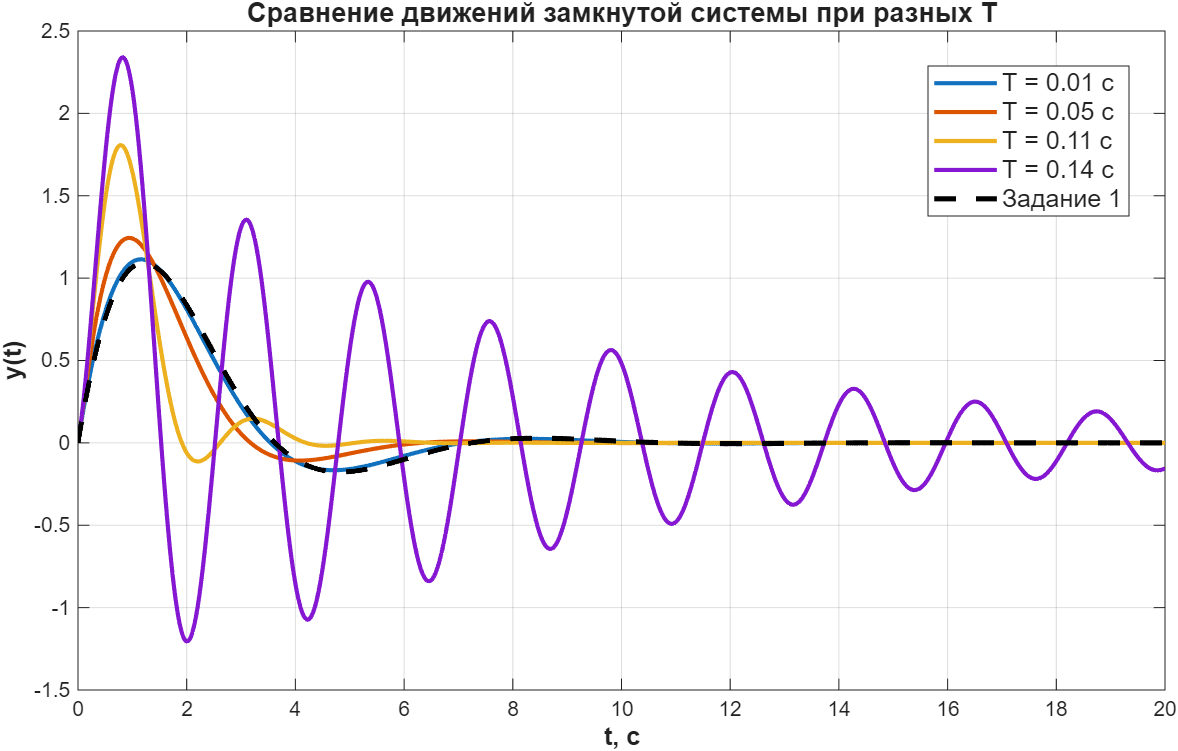
\includegraphics[width=0.8\linewidth]{images/Figure_4_2_5.png}
    \caption{График сравнения движений замкнутой системы при разных $T$}
    \label{fig:placeholder}
\end{figure}

\subsection{Выводы}

Во втором задании "идеальное" дифференцирующее звено было заменено на реальное, описанное передаточной функцией

\[
W(s) = \frac{s}{Ts + 1},
\]

Аналитически, с использованием критерия Гурвица, был определён диапазон значений
параметра $T$, при которых система остаётся асимптотически устойчивой.

Моделирование показало, что при малых значениях $T$ поведение системы
близко к реализации "идеального" дифференцирующего звена, и переходный процесс
является быстро затухающим. С увеличением $T$ качество переходного процесса
ухудшается: возрастает колебательность и время установления.
При приближении $T$ к критическому значению система становится близкой
к границе устойчивости.






\newpage

\section{Задание 3. Задача слежения для системы с астатизмом нулевого порядка (П-регулятор)}

\subsection{Исходные данные}

\begin{figure}[H]
    \centering
    \includegraphics[width=0.6\linewidth]{images/image_4_3_1.png}
    \caption{Общий вид замкнутой системы}
    \label{fig:placeholder1}
\end{figure}

Рассмотрим замкнутую систему, заданную структурной схемой на рисунке \ref{fig:placeholder1}, где:

$$
H(s)=k
$$

Берем передаточную функцию в соответсвии с вариантом:

$$
W(s)=\dfrac{4}{s^2+s+3}
$$

Характеристики задающегося воздейстаия $g(t)$ также берем в соответсвии с вариантом:

\begin{table}[H]
    \centering
    \renewcommand{\arraystretch}{2} % увеличивает высоту строк
    \begin{tabular}{|c|c|c|c|}
    \hline
        $A$ & $Vt$ & $\dfrac{at^2}{2}$ & $A\sin(\omega t)$ \\[3pt] \hline
        $1$ & $3t$ & $0.5t^2$ & $\sin(0.5t)$ \\ \hline
    \end{tabular}
    \label{tab:placeholder}
\end{table}

\subsection{Аналитические расчеты}

\subsubsection{Выбор параметров $k$}

Ошибка задаётся уравнением:

$$
E(s)=G(s)-Y(s)
$$

Регулятор задаётся уравнением:

$$
U(s)=H(s)\cdot E(s)
$$

Объект задаётся уравнением:

$$
Y(s)=W(s)\cdot U(s)
$$

После подстановки получаем:

$$
Y(s)=W(s)\cdot H(s) \cdot E(s)=W(s)\cdot H(s) \cdot (G(s)-Y(s))
$$

$$
Y(s)+Y(s)\cdot W(s)\cdot H(s)=W(s)\cdot H(s)\cdot G(s)
$$

Таким образом передаточная функция замкнутой системы:

$$
W_{\text{раз}}(s)=\dfrac{Y(s)}{G(s)}= \dfrac{W(s)\cdot H(s)}{1+W(s)\cdot H(s)}
$$

Подставляя значения из нашего варианта получаем:

$$
W_{\text{раз}}(s)=\dfrac{k\cdot \dfrac{4}{s^2+s+3}}{1+k\cdot \dfrac{4}{s^2+s+3}}=\dfrac{4k}{s^2+s+3+4k}
$$

Характеристическое уравнение будет иметь вид:

$$
\lambda^2+\lambda+3+4k=0
$$

Система будет ассимптотически устойчива при выполнении критерия Гурвинца:

$$
\begin{cases}
    1>0\\
    1>0\\
    3+4k>0
\end{cases}
$$

Получаем что система будет ассимптотически устойчива при $k>-\dfrac{3}{4}$

Выбирем следующие $k$:

$$
k_1=-\dfrac{1}{2} \qquad k_2=1 \qquad k=10
$$

\subsubsection{Вычисление установленной ошибки}

Передаточная функция по ошибке имеет вид:

$$
W_e(s)=\dfrac{E(s)}{G(s)}=\dfrac{1}{1+W(s)H(s)}=\dfrac{s^2+s+3}{s^2+s+3+4k}
$$

Установившаяся ошибка:

$$
e_{\text{уст}}=\lim \limits_{t\to\infty}{e(t)}=\lim \limits_{s\to0}{sE(s)}=\lim \limits_{s\to0}{s\cdot W_e(s)\cdot G(s)}
$$

Для $g(t)=1$:

$$
e_{\text{уст}}=\lim \limits_{s\to0}{s\cdot \dfrac{s^2+s+3}{s^2+s+3+4k}\cdot \dfrac{1}{s}}=\dfrac{3}{3+4k}
$$

При $k_{1,2,3}$:

\begin{itemize}
    \item При $k=-0,5$: $e_{\text{уст}}=\dfrac{3}{3-2}=3$
    \item При $k=1$: $e_{\text{уст}}=\dfrac{3}{3+4}=\dfrac{3}{7}$
    \item При $k=10$: $e_{\text{уст}}=\dfrac{3}{3+40}=\dfrac{3}{43}$
\end{itemize}


\subsection{Структурная схема}

\begin{figure}
    \centering
    \includegraphics[width=0.75\linewidth]{images/image_4_3_2.png}
    \caption{Структурная схема системы с П-регулятором}
    \label{fig:placeholder}
\end{figure}

\subsection{Графики выходов}

\begin{figure}[H]
    \centering
    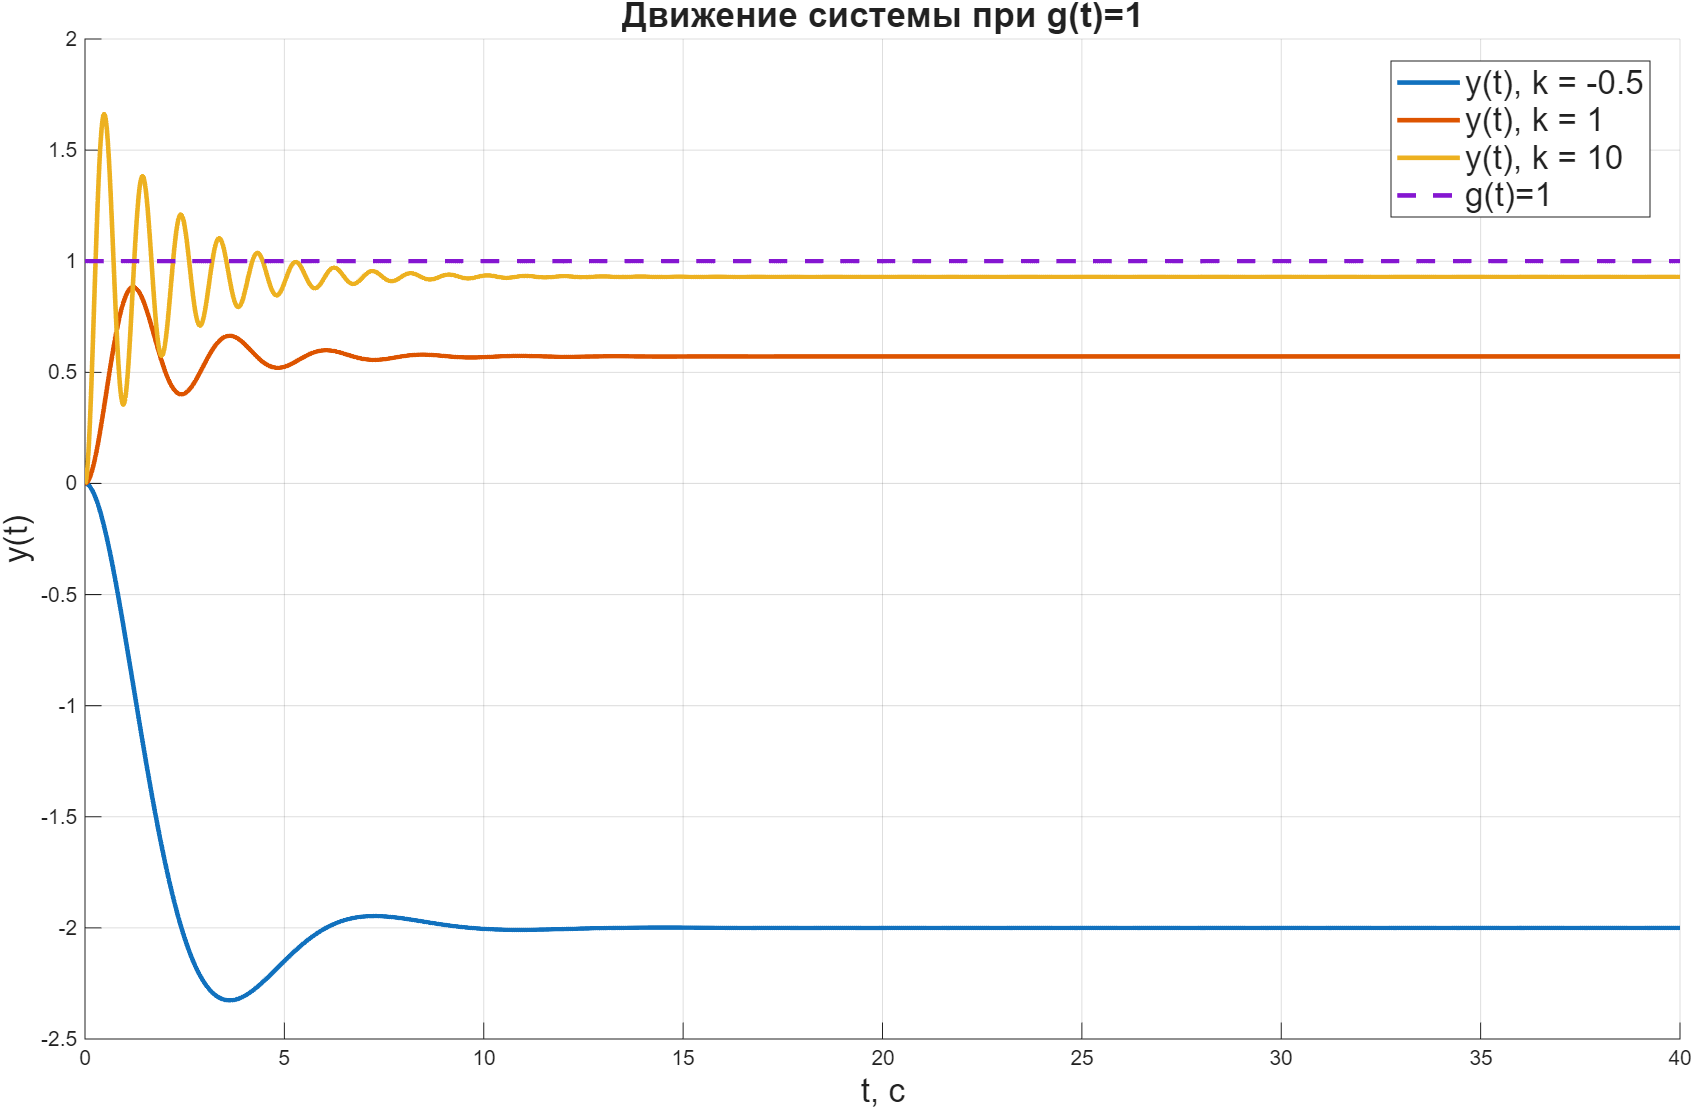
\includegraphics[width=0.75\linewidth]{images/Figure_4_3_1.png}
    \caption{Сопоставление движений системы при $g(t)=1$}
    \label{fig:placeholder}
\end{figure}

\begin{figure}[H]
    \centering
    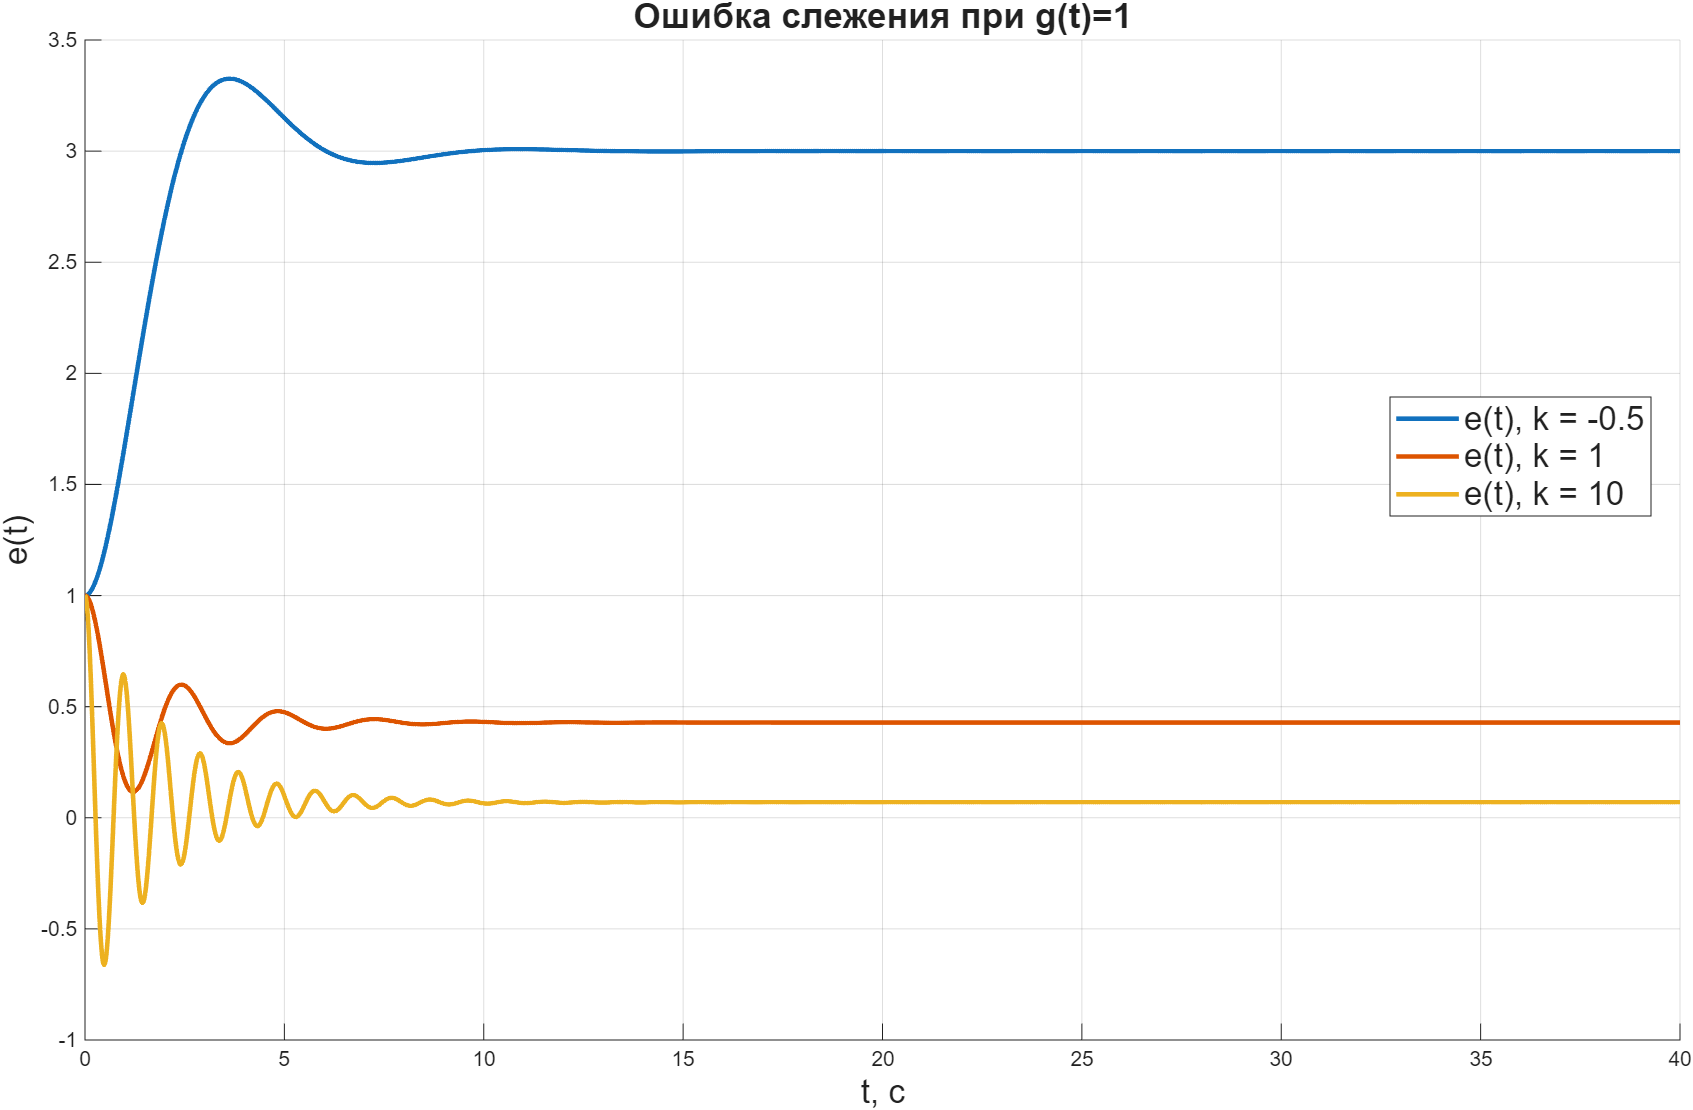
\includegraphics[width=0.75\linewidth]{images/Figure_4_3_2.png}
    \caption{Сопоставление ошибок системы при $g(t)=1$}
    \label{fig:placeholder}
\end{figure}

\begin{figure}[H]
    \centering
    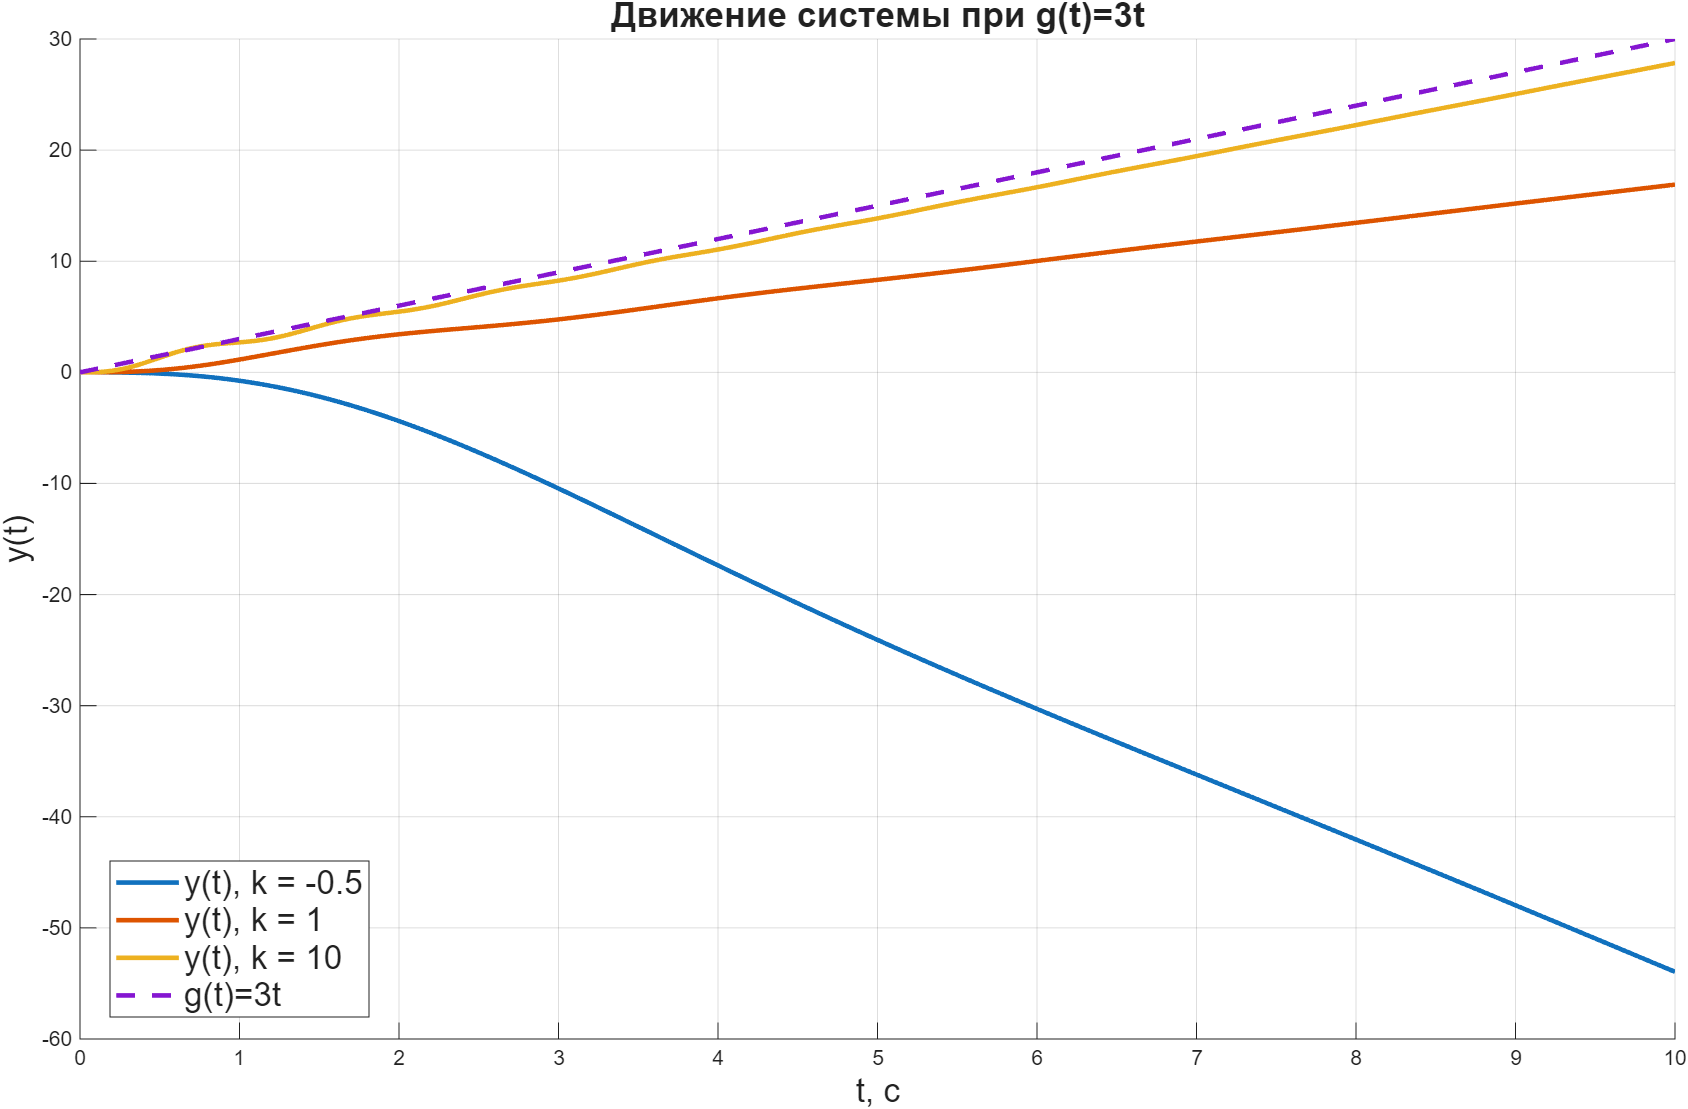
\includegraphics[width=0.75\linewidth]{images/Figure_4_3_3.png}
    \caption{Сопоставление движений системы при $g(t)=3t$}
    \label{fig:placeholder}
\end{figure}

\begin{figure}[H]
    \centering
    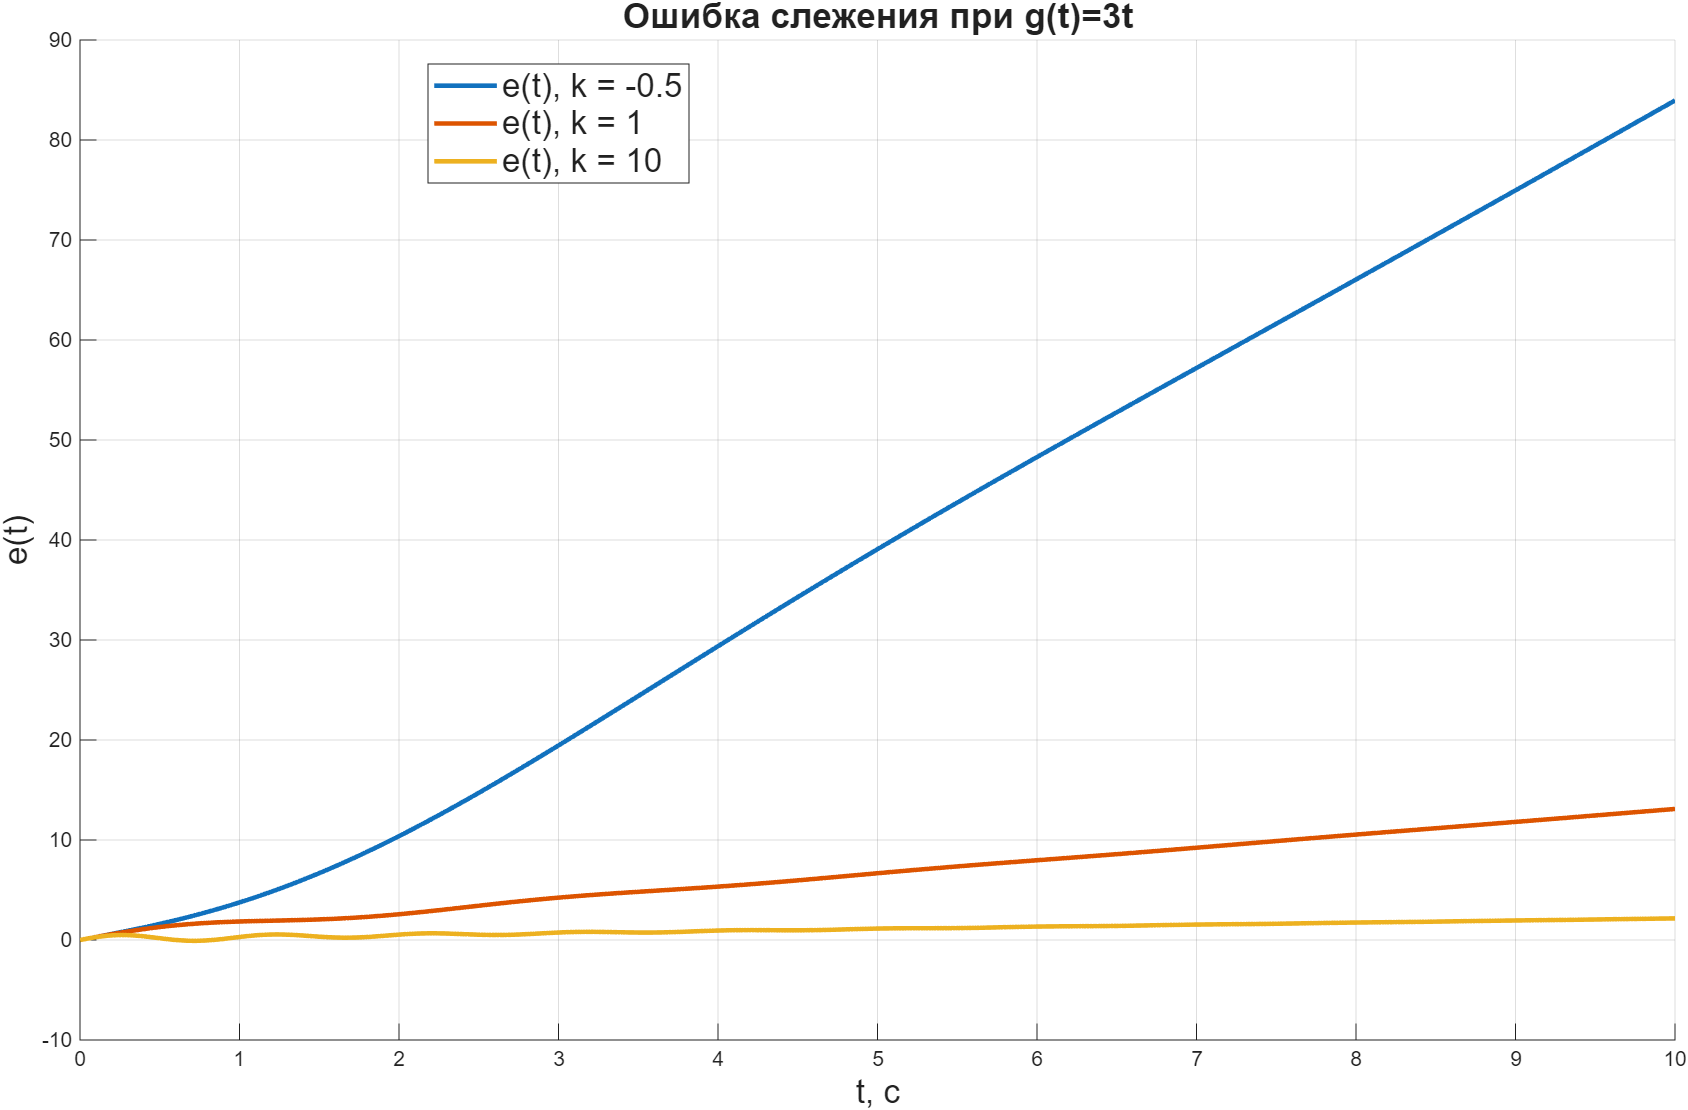
\includegraphics[width=0.75\linewidth]{images/Figure_4_3_4.png}
    \caption{Сопоставление ошибок системы при $g(t)=3t$}
    \label{fig:placeholder}
\end{figure}

\subsection{Выводы}

В третьем задании была рассмотрена система слежения с астатизмом нулевого порядка,
в которой в качестве регулятора использовался пропорциональный закон управления
$H(s) = k$.

Исследование стационарного режима при $g(t)=A$ показало, что система
обладает конечной установившейся ошибкой
\[
e_{\text{уст}} = \frac{3}{3+4k},
\]
которая уменьшается с ростом коэффициента усиления $k$.
Результаты моделирования полностью подтвердили аналитические расчёты:
при увеличении $k$ выход системы быстрее приближается к задающему воздействию,
а величина установившейся ошибки уменьшается.

В режиме движения с постоянной скоростью $g(t)=Vt$ установившаяся ошибка
оказалась бесконечной, что свидетельствует о неспособности системы с
астатизмом нулевого порядка обеспечивать точное слежение за линейно
возрастающим сигналом.

Таким образом, пропорциональный регулятор обеспечивает устойчивость и позволяет
уменьшить статическую ошибку при постоянном воздействии, однако система с
астатизмом нулевого порядка не способна обеспечить слежение без ошибки за
сигналами с ненулевой скоростью изменения. Для устранения этой проблемы
необходимо повышение порядка астатизма системы.




\newpage

\section{Задание 4. Задача слежения для системы с астатизмом первого порядка (И-регулятор)}

\subsection{Исходные данные}

Рассмотрим замкнутую систему, заданную структурной схемой на рисунке \ref{fig:placeholder1}, где:

$$
H(s)=\dfrac{k}{s}
$$

Берем передаточную функцию в соответсвии с вариантом:

$$
W(s)=\dfrac{4}{s^2+s+3}
$$

Характеристики задающегося воздейстаия $g(t)$ также берем в соответсвии с вариантом:

\begin{table}[H]
    \centering
    \renewcommand{\arraystretch}{2} % увеличивает высоту строк
    \begin{tabular}{|c|c|c|c|}
    \hline
        $A$ & $Vt$ & $\dfrac{at^2}{2}$ & $A\sin(\omega t)$ \\[3pt] \hline
        $1$ & $3t$ & $0.5t^2$ & $\sin(0.5t)$ \\ \hline
    \end{tabular}
    \label{tab:placeholder}
\end{table}

\subsection{Аналитические расчеты}

\subsubsection{Выбор параметров $k$}

Передаточная функция замкнутой системы:

$$
W_{\text{раз}}(s)=\dfrac{Y(s)}{G(s)}= \dfrac{W(s)\cdot H(s)}{1+W(s)\cdot H(s)}
$$

Подставляя значения из нашего варианта получаем:

$$
W_{\text{раз}}(s)=\dfrac{\dfrac{k}{s}\cdot \dfrac{4}{s^2+s+3}}{1+\dfrac{k}{s}\cdot \dfrac{4}{s^2+s+3}}=\dfrac{4k}{s^3+s^2+3s+4k}
$$

Характеристическое уравнение будет иметь вид:

$$
\lambda^3+\lambda^2+3\lambda+4k=0
$$

Система будет ассимптотически устойчива при выполнении критерия Гурвинца:

$$
\begin{cases}
    4k>0\\
    3>0\\
    1>0\\
    3>4k
\end{cases}
$$

Получаем что система будет ассимптотически устойчива при $0<k<0.75$

Выбирем следующие $k$:

$$
k_1=0.1 \qquad k_2=0.4 \qquad k=0.6
$$

\subsubsection{Вычисление установленной ошибки}

Передаточная функция по ошибке имеет вид:

$$
W_e(s)=\dfrac{E(s)}{G(s)}=\dfrac{1}{1+W(s)H(s)}=\dfrac{s^3+s^2+3s}{s^3+s^2+3s+4k}
$$

Установившаяся ошибка:

$$
e_{\text{уст}}=\lim \limits_{t\to\infty}{e(t)}=\lim \limits_{s\to0}{sE(s)}=\lim \limits_{s\to0}{s\cdot W_e(s)\cdot G(s)}
$$

Для $g(t)=1$:

$$
e_{\text{уст}}=\lim \limits_{s\to0}{s\cdot \dfrac{s^3+s^2+3s}{s^3+s^2+3s+4k}\cdot \dfrac{1}{s}}=0
$$

При $k_{1,2,3}$:

\begin{itemize}
    \item При $k=0.1$: $e_{\text{уст}}=0$
    \item При $k=0.4$: $e_{\text{уст}}=0$
    \item При $k=0.6$: $e_{\text{уст}}=0$
\end{itemize}

Для $g(t)=3t$

$$
e_{\text{уст}}=\lim \limits_{s\to0}{s\cdot \dfrac{s^3+s^2+3s}{s^3+s^2+3s+4k}\cdot \dfrac{3}{s^2}}=\dfrac{9}{4k}
$$

При $k_{1,2,3}$:

\begin{itemize}
    \item При $k=0.1$: $e_{\text{уст}}=22.5$
    \item При $k=0.4$: $e_{\text{уст}}=5.625$
    \item При $k=0.6$: $e_{\text{уст}}=3.75$
\end{itemize}


\subsection{Структурная схема}

\begin{figure}
    \centering
    \includegraphics[width=0.75\linewidth]{images/image_4_4_1.png}
    \caption{Структурная схема системы с И-регулятором}
    \label{fig:placeholder}
\end{figure}

\subsection{Графики выходов}

\begin{figure}[H]
    \centering
    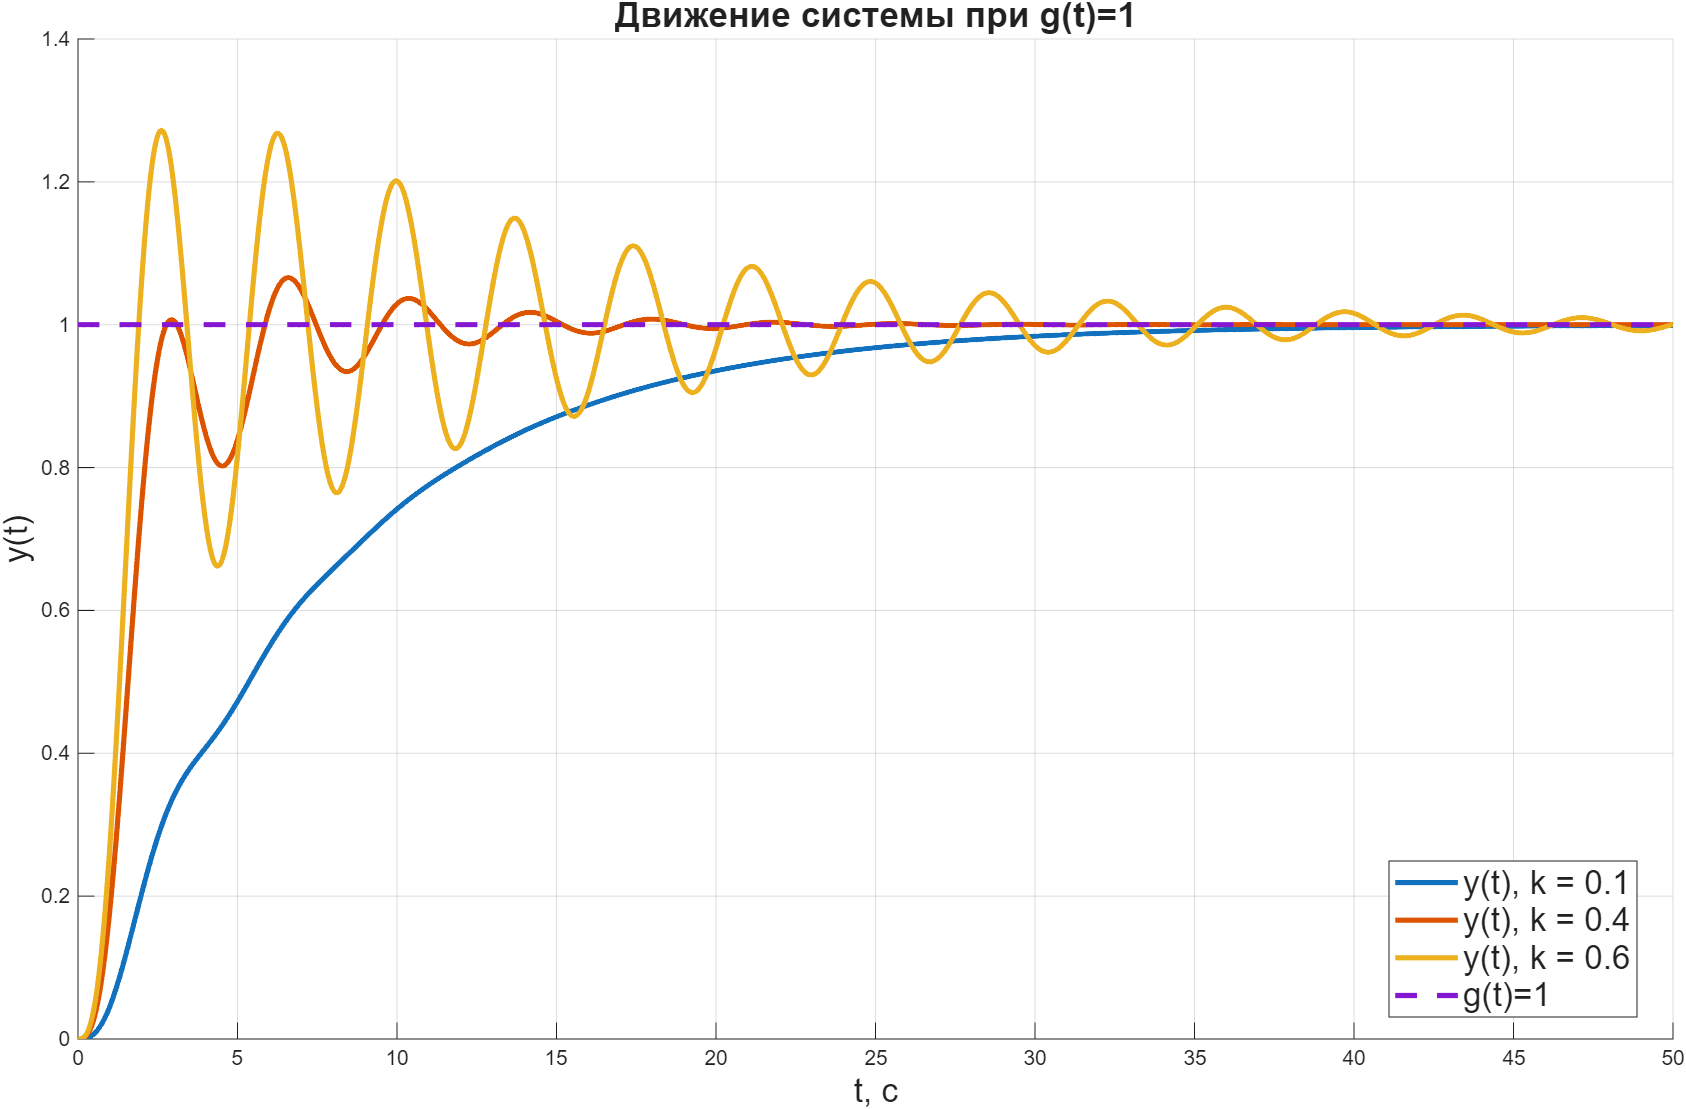
\includegraphics[width=0.75\linewidth]{images/Figure_4_4_1.png}
    \caption{Сопоставление движений системы при $g(t)=1$}
    \label{fig:placeholder}
\end{figure}

\begin{figure}[H]
    \centering
    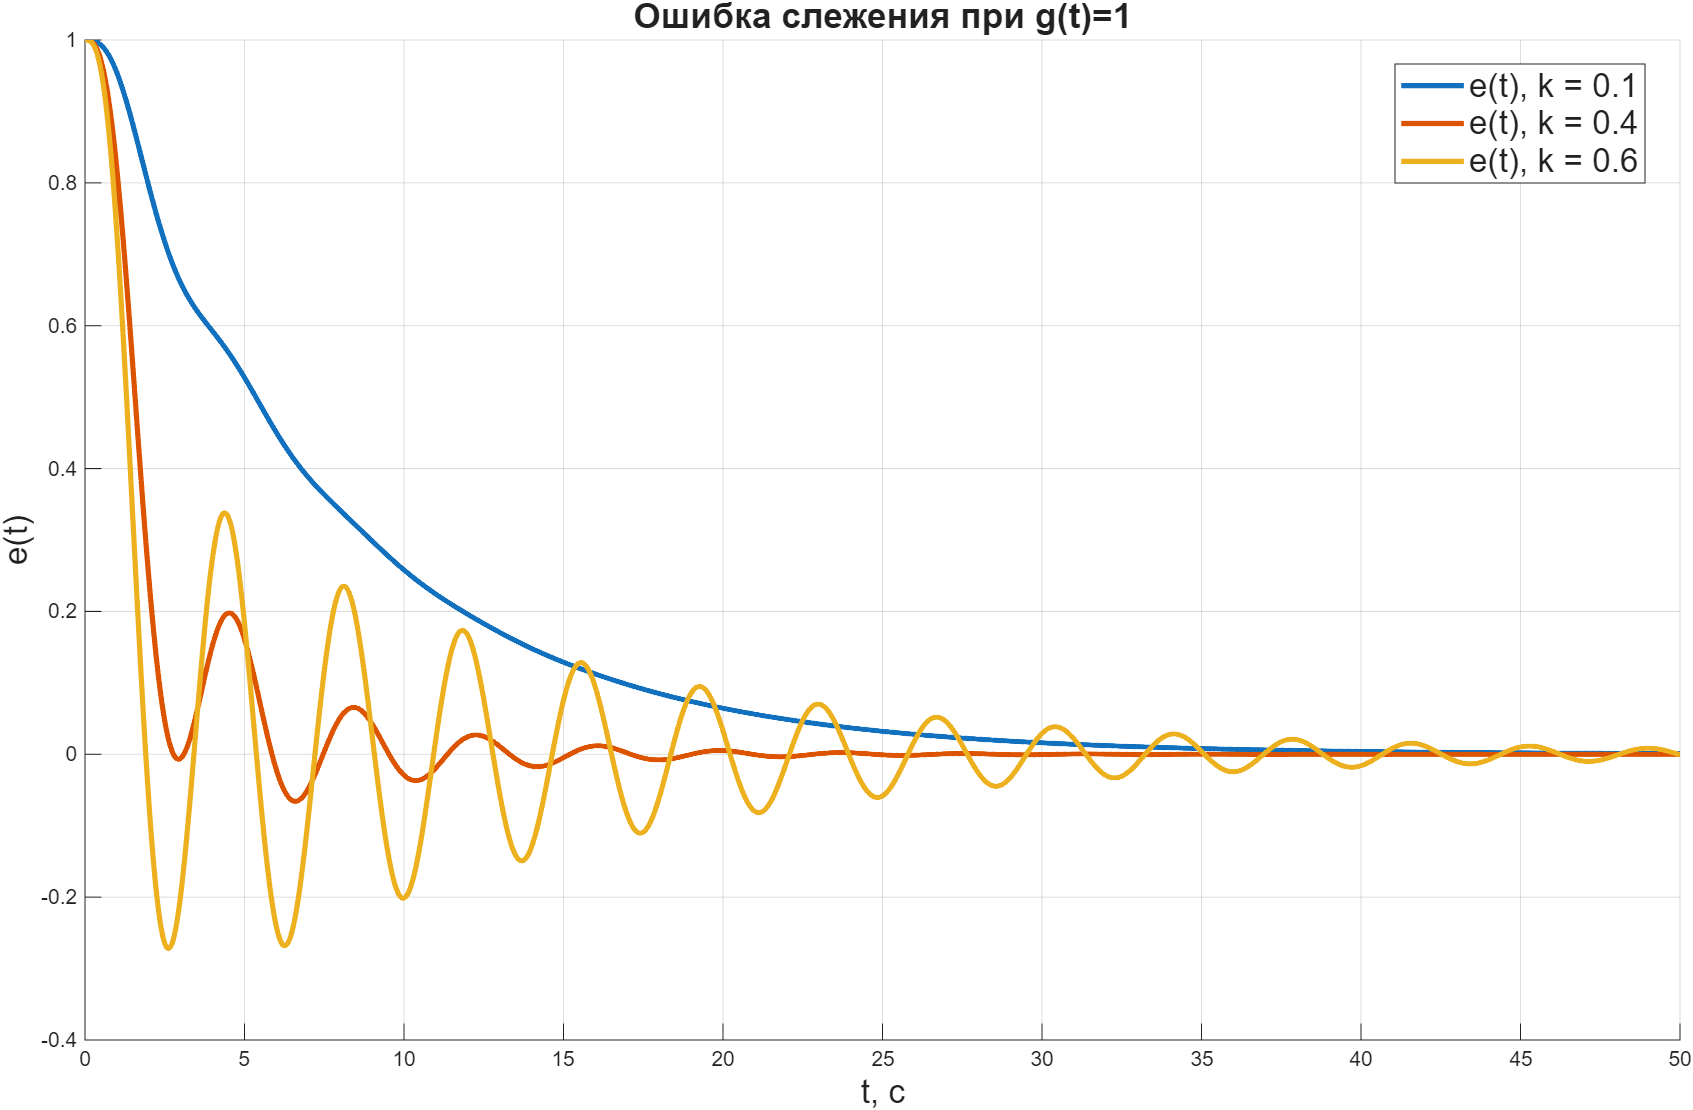
\includegraphics[width=0.75\linewidth]{images/Figure_4_4_2.png}
    \caption{Сопоставление ошибок системы при $g(t)=1$}
    \label{fig:placeholder}
\end{figure}

\begin{figure}[H]
    \centering
    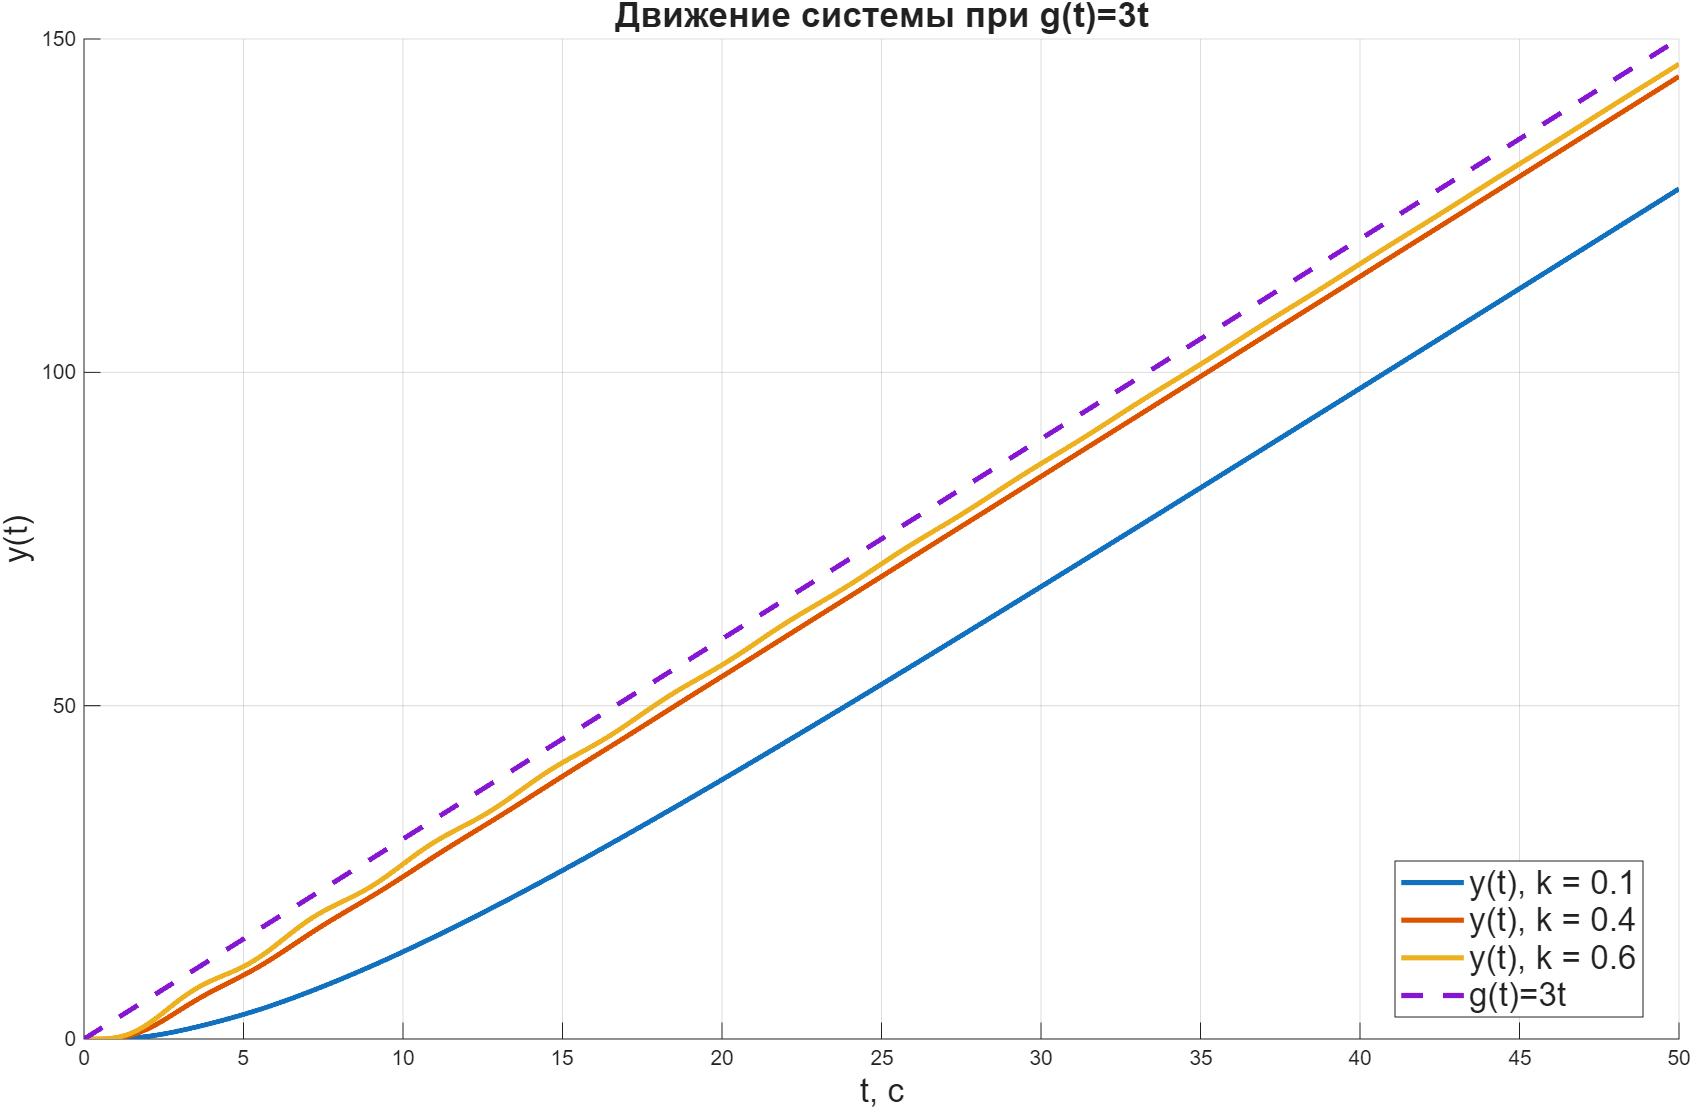
\includegraphics[width=0.75\linewidth]{images/Figure_4_4_3.png}
    \caption{Сопоставление движений системы при $g(t)=3t$}
    \label{fig:placeholder}
\end{figure}

\begin{figure}[H]
    \centering
    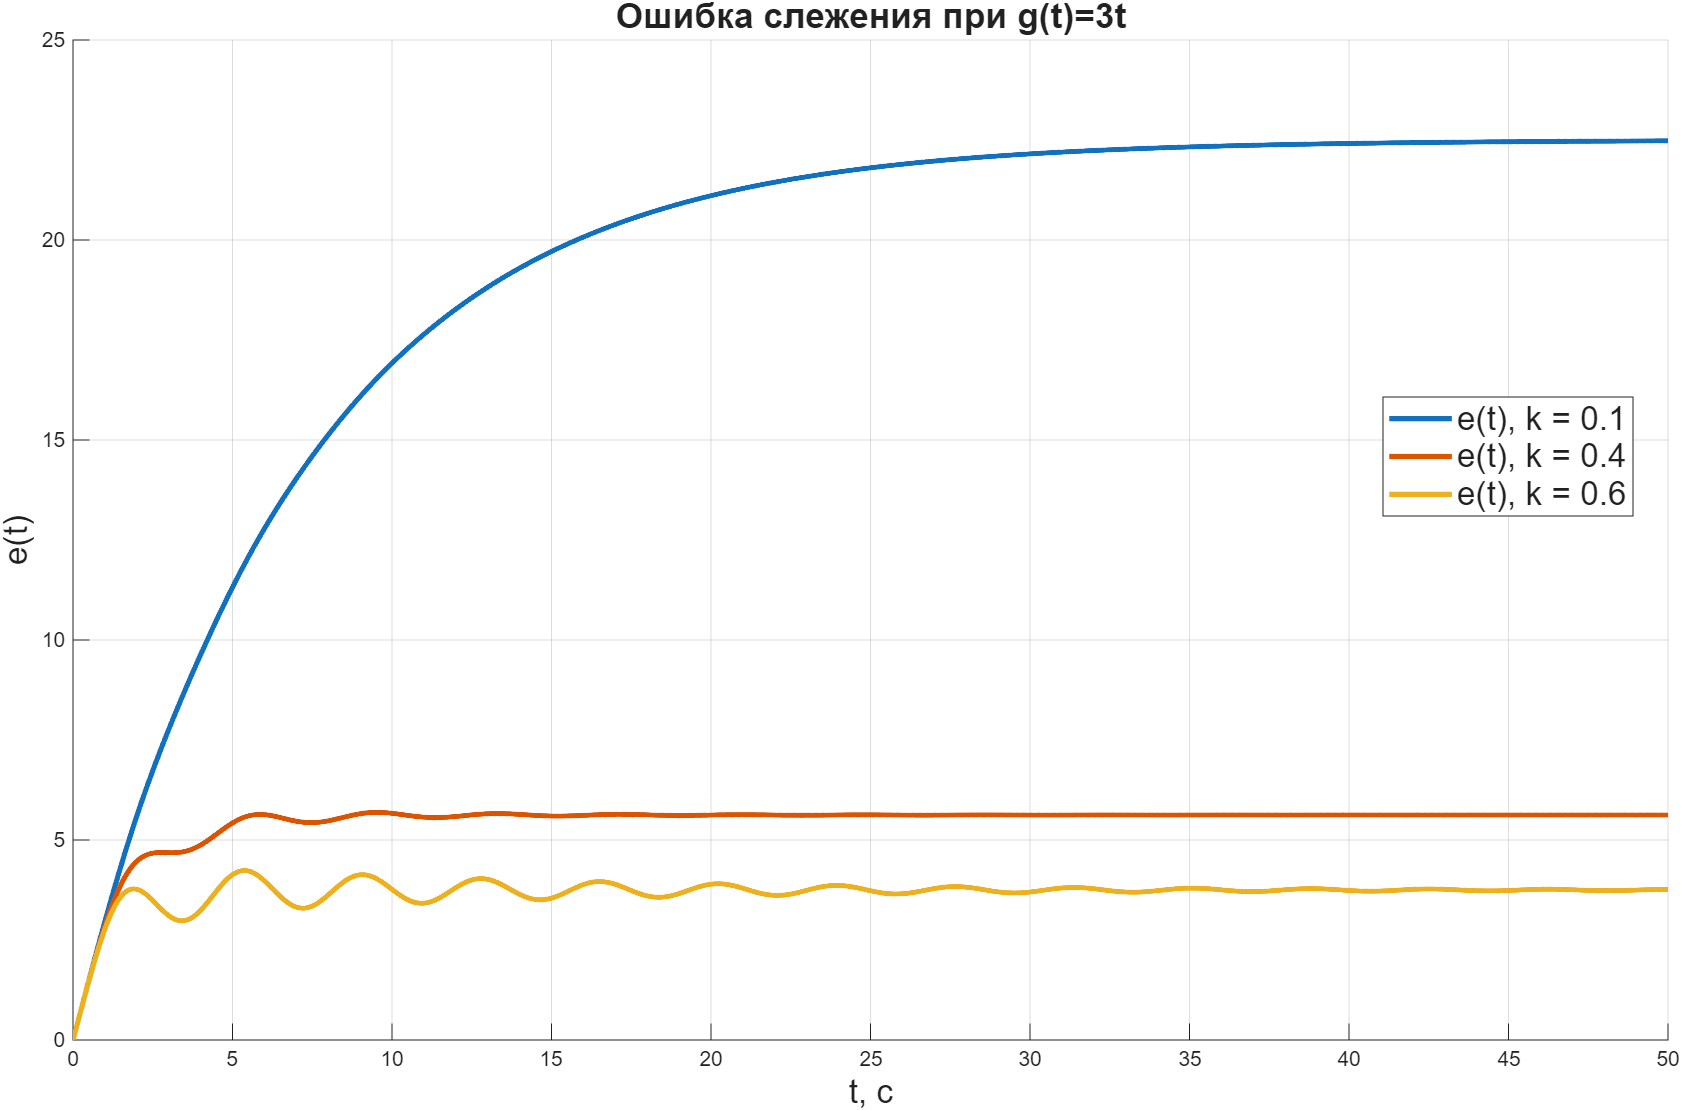
\includegraphics[width=0.75\linewidth]{images/Figure_4_4_4.png}
    \caption{Сопоставление ошибок системы при $g(t)=3t$}
    \label{fig:placeholder}
\end{figure}

\begin{figure}[H]
    \centering
    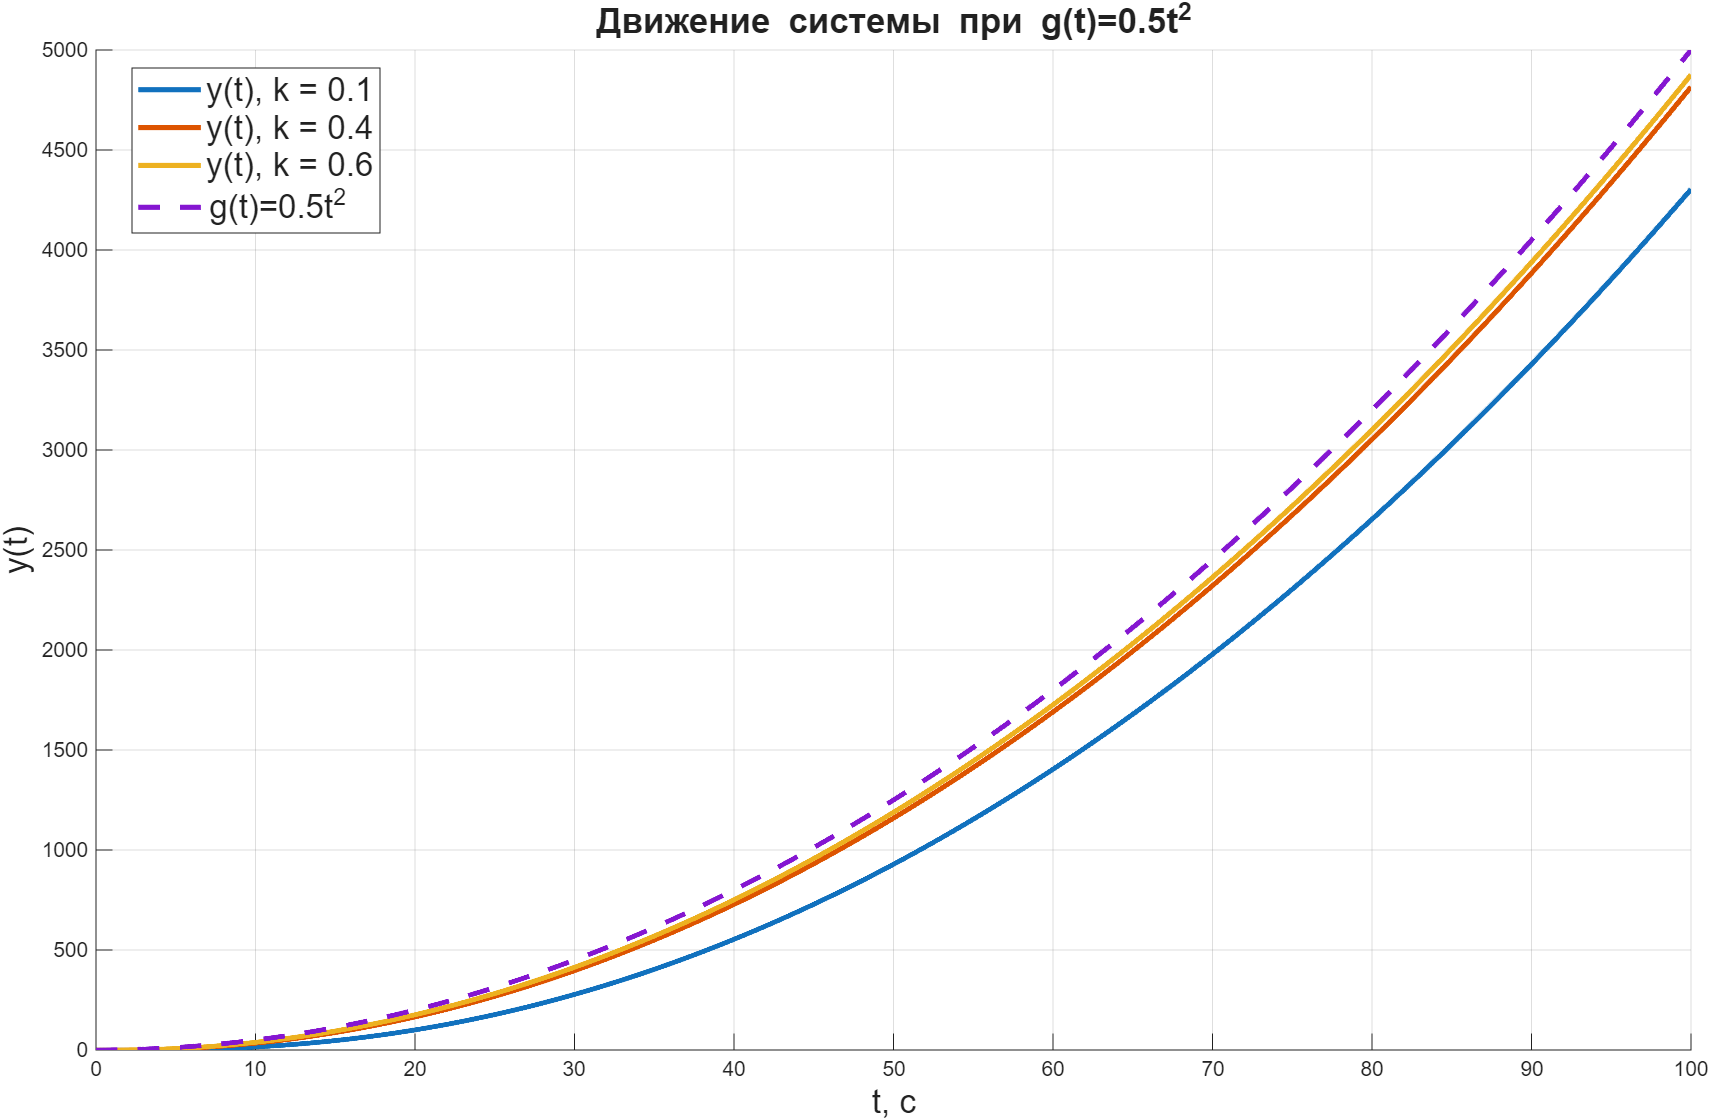
\includegraphics[width=0.75\linewidth]{images/Figure_4_4_5.png}
    \caption{Сопоставление движений системы при $g(t)=0.5t^2$}
    \label{fig:placeholder}
\end{figure}

\begin{figure}[H]
    \centering
    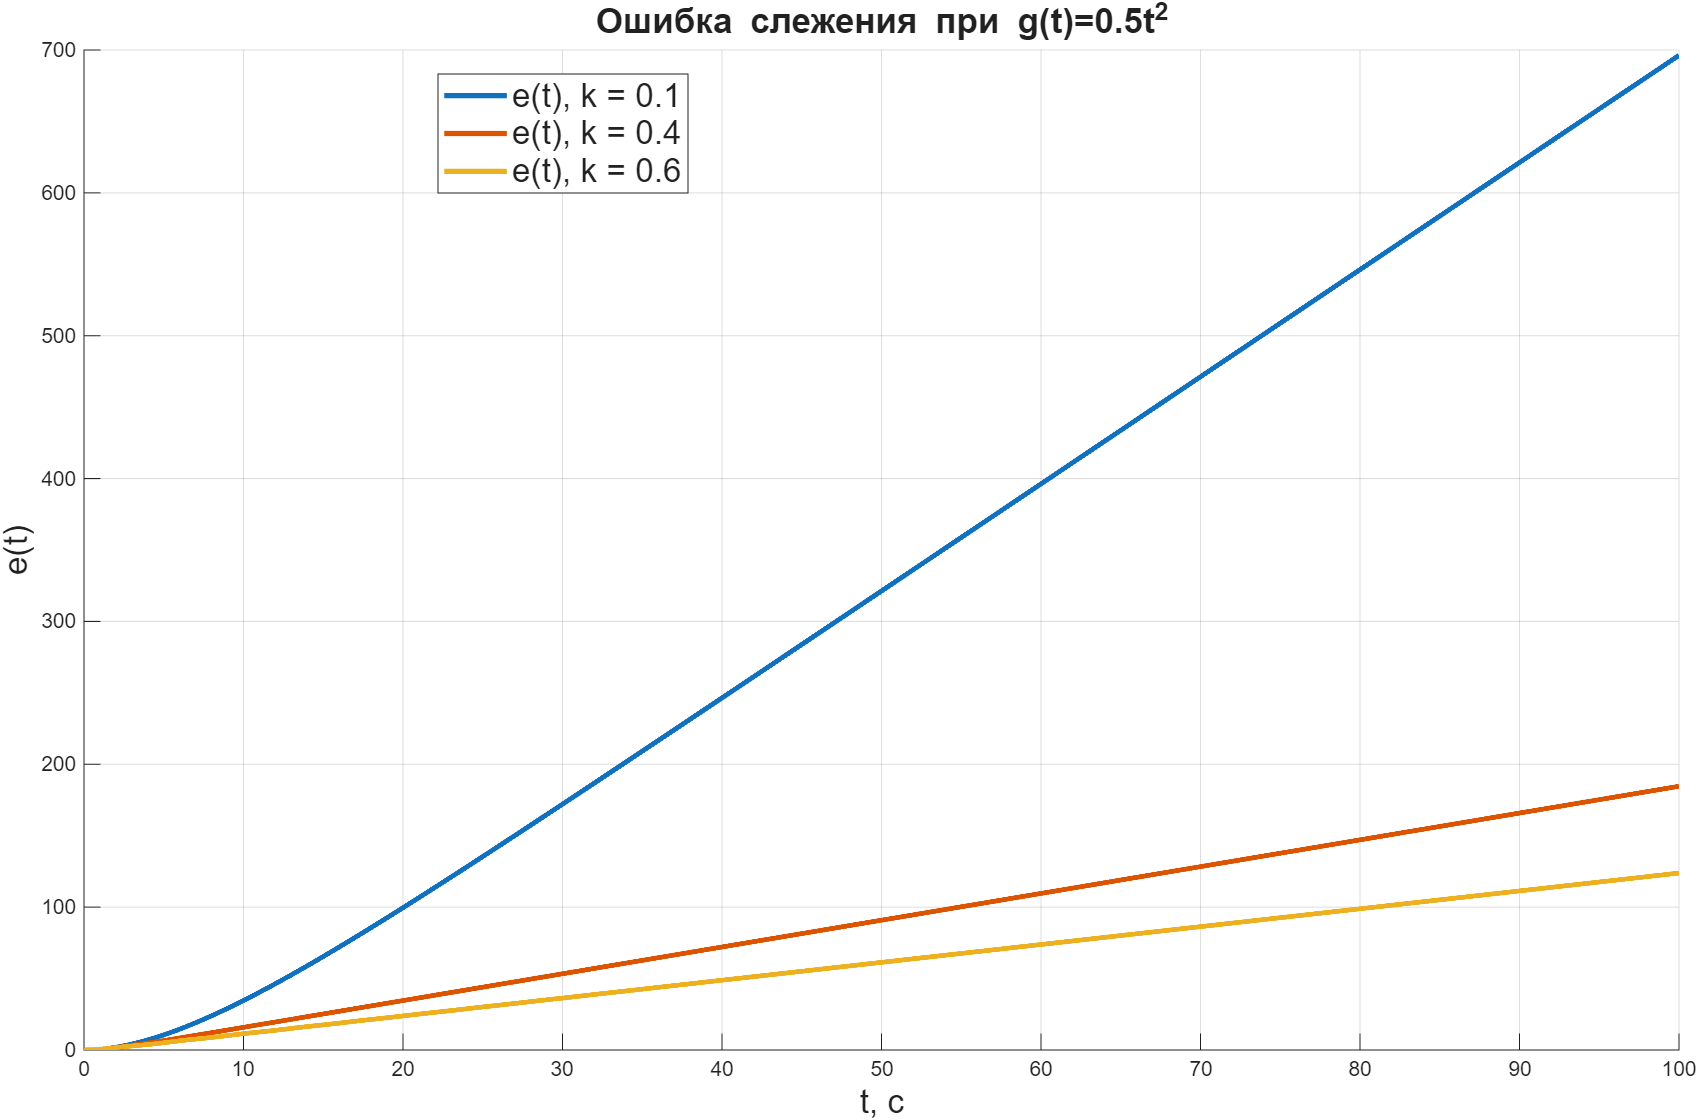
\includegraphics[width=0.75\linewidth]{images/Figure_4_4_6.png}
    \caption{Сопоставление ошибок системы при $g(t)=0.5t^2$}
    \label{fig:placeholder}
\end{figure}

\subsection{Выводы}

В четвёртом задании была рассмотрена система слежения с астатизмом первого порядка,
в которой использовался интегральный регулятор
\[
H(s)=\frac{k}{s}.
\]

В стационарном режиме при $g(t)=A$ установившаяся ошибка равна нулю:
\[
e_{\text{уст}} = 0,
\]
что подтверждает наличие астатизма первого порядка. Результаты моделирования
показали полное совпадение аналитических и численных данных.

В режиме движения с постоянной скоростью $g(t)=Vt$ установившаяся ошибка
оказалась конечной и равной
\[
e_{\text{уст}} = \frac{9}{4k},
\]
то есть уменьшается при увеличении коэффициента $k$.
Таким образом, система способна обеспечивать слежение за линейно
возрастающим сигналом с конечной ошибкой.

В режиме движения с постоянным ускорением $g(t)=\frac{at^2}{2}$ ошибка
оказалась неограниченно возрастающей, что свидетельствует о том,
что система первого порядка астатизма не способна обеспечивать
точное слежение за квадратичным сигналом.

Таким образом, введение интегрального звена увеличивает порядок астатизма
системы и устраняет статическую ошибку при постоянном воздействии,
однако для точного слежения за сигналами более высокого порядка
необходимо дальнейшее повышение порядка астатизма.


\newpage

\section{Задание 5. Задача слежения для системы с астатизмом первого порядка (ПИ-регулятор)}

\subsection{Исходные данные}

Рассмотрим замкнутую систему, заданную структурной схемой на рисунке \ref{fig:placeholder1}, где:

$$
H(s)=\dfrac{k_{\text{И}}}{s}+k_{\text{П}}
$$

Берем передаточную функцию в соответсвии с вариантом:

$$
W(s)=\dfrac{4}{s^2+s+3}
$$

Характеристики задающегося воздейстаия $g(t)$ также берем в соответсвии с вариантом:

\begin{table}[H]
    \centering
    \renewcommand{\arraystretch}{2} % увеличивает высоту строк
    \begin{tabular}{|c|c|c|c|}
    \hline
        $A$ & $Vt$ & $\dfrac{at^2}{2}$ & $A\sin(\omega t)$ \\[3pt] \hline
        $1$ & $3t$ & $0.5t^2$ & $\sin(0.5t)$ \\ \hline
    \end{tabular}
    \label{tab:placeholder}
\end{table}

\subsection{Аналитические расчеты}

\subsubsection{Выбор параметров $k_{\text{И}}$ и $k_{\text{П}}$}

Передаточная функция замкнутой системы:

$$
W_{\text{раз}}(s)=\dfrac{Y(s)}{G(s)}= \dfrac{W(s)\cdot H(s)}{1+W(s)\cdot H(s)}
$$

Подставляя значения из нашего варианта получаем:

$$
W_{\text{раз}}(s)=\dfrac{\left(k_{\text{П}}+\dfrac{k_{\text{И}}}{s}\right)\cdot \dfrac{4}{s^2+s+3}}{1+\left(k_{\text{П}}+\dfrac{k_{\text{И}}}{s}\right)\cdot \dfrac{4}{s^2+s+3}}=\dfrac{4sk_{\text{П}}+4k_{\text{И}}}{s^3+s^2+3s+4sk_{\text{П}}+4k_{\text{И}}}
$$

Характеристическое уравнение будет иметь вид:

$$
\lambda^3+\lambda^2+3\lambda+4\lambda k_{\text{П}}+4k_{\text{И}}=0
$$

Система будет ассимптотически устойчива при выполнении критерия Гурвинца:

$$
\begin{cases}
    4k_{\text{И}}>0\\
    3+4k_{\text{П}}>0\\
    1>0\\
    3+4k_{\text{П}}>4k_{\text{И}}
\end{cases}
$$

Получаем что система будет ассимптотически устойчива при:

$$
\begin{cases}
    k_{\text{И}}>0\\
    k_{\text{П}}>-\dfrac{3}{4}\\
    3+4k_{\text{П}}>4k_{\text{И}}
\end{cases}
$$

Выбирем следующие $k_{\text{П}}$ и $k_{\text{И}}$:

$$
(k_{\text{П}}, k_{\text{И}}) =\{(5,\; 0.5), \
(5,\; 4), \
(10,\; 0.5), \
(10,\; 4)\}
$$

\subsubsection{Вычисление установленной ошибки}

Передаточная функция ошибки:

$$
W_e(s)=\dfrac{s^3+s^2+3s}{s^3+s^2+3s+4sk_{\text{П}}+4k_{\text{И}}}
$$

Установившаяся ошибка:

$$
e_{\text{уст}}=\lim \limits_{t\to\infty}{e(t)}=\lim \limits_{s\to0}{sE(s)}=\lim \limits_{s\to0}{s\cdot W_e(s)\cdot G(s)}
$$

Для $g(t)=3t$

$$
e_{\text{уст}}=\lim_{s\to0}
s\cdot\dfrac{s^3+s^2+3s}{s^3+s^2+3s+4sk_{\text{П}}+4k_{\text{И}}}
\cdot\dfrac{3}{s^2}
=\dfrac{9}{4k_{\text{И}}}
$$

При разных $k_{\text{И}}$:

\begin{itemize}
    \item При $k_{\text{И}}=4$: $e_{\text{уст}}=\dfrac{9}{8}=1.125$
    \item При $k_{\text{И}}=0.5$: $e_{\text{уст}}=\dfrac{9}{2}=4.5$
\end{itemize}

\subsection{Структурная схема}

\begin{figure}
    \centering
    \includegraphics[width=0.75\linewidth]{images/image_4_5_1.png}
    \caption{Структурная схема системы с ПИ-регулятором}
    \label{fig:placeholder}
\end{figure}

\subsection{Графики выходов}

\begin{figure}[H]
    \centering
    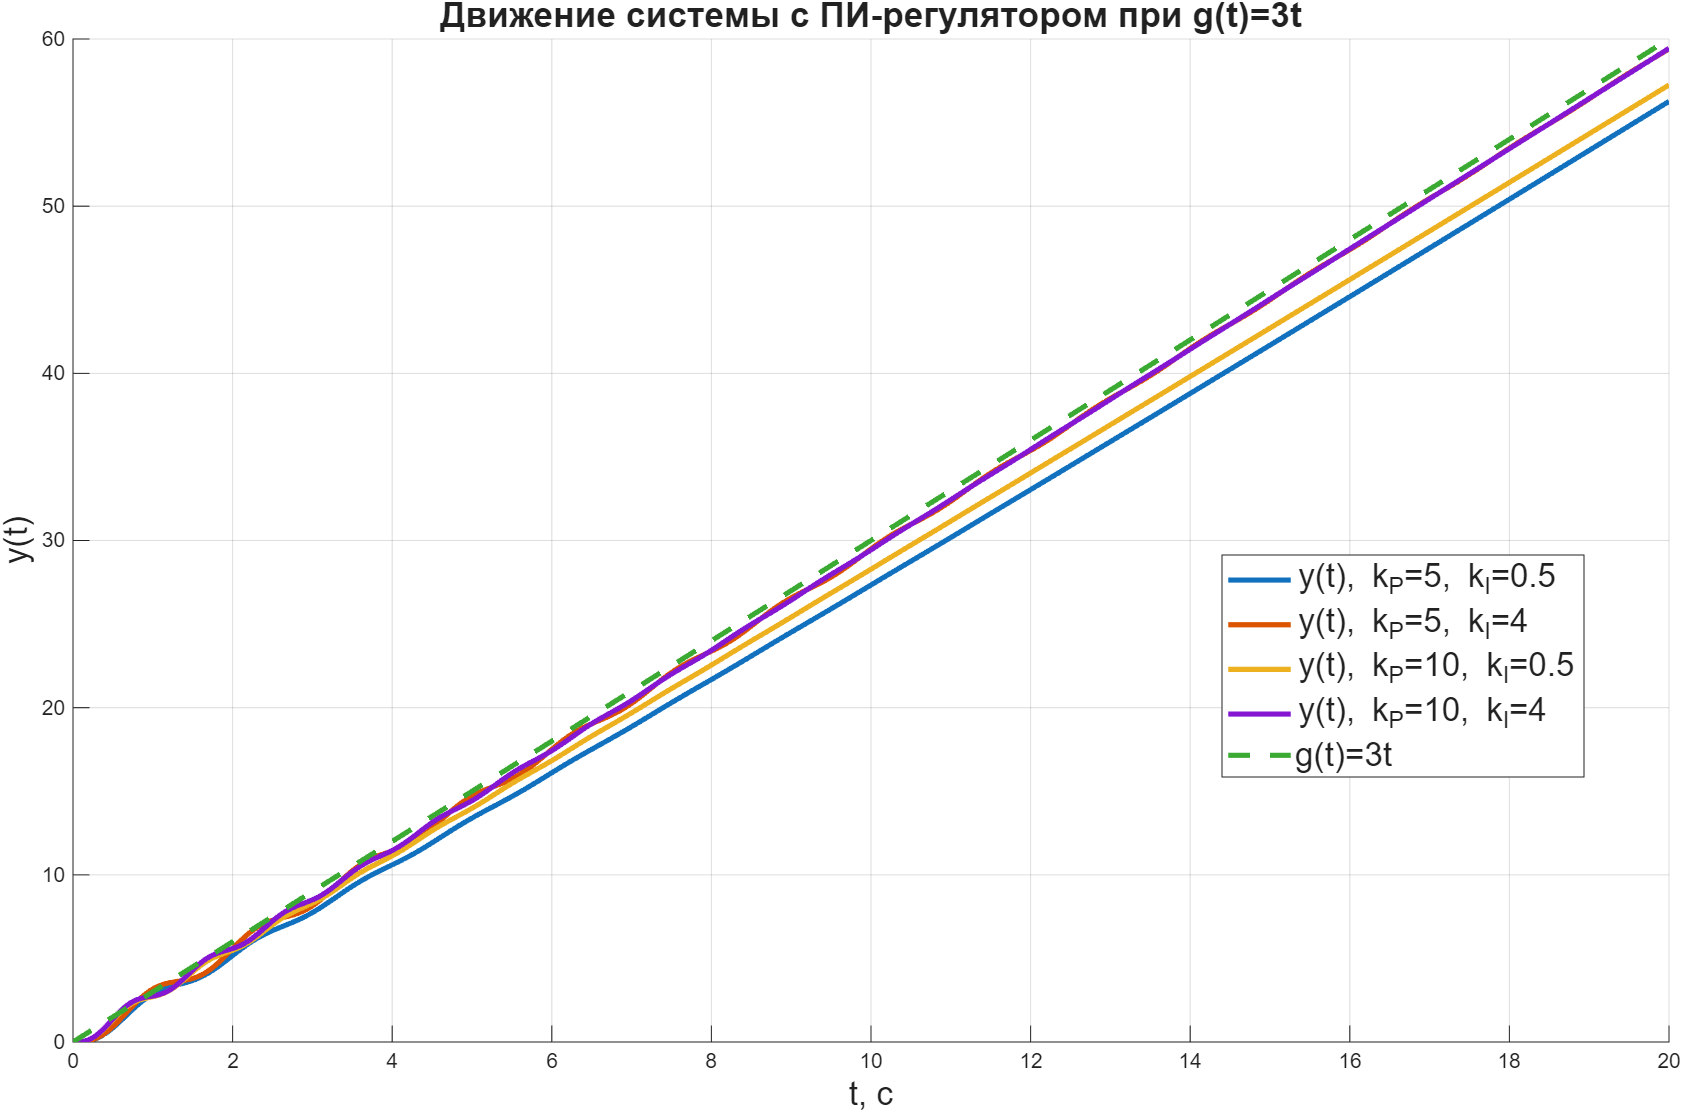
\includegraphics[width=0.75\linewidth]{images/Figure_4_5_1.png}
    \caption{Сопоставление движений системы при $g(t)=3t$}
    \label{fig:placeholder}
\end{figure}

\begin{figure}[H]
    \centering
    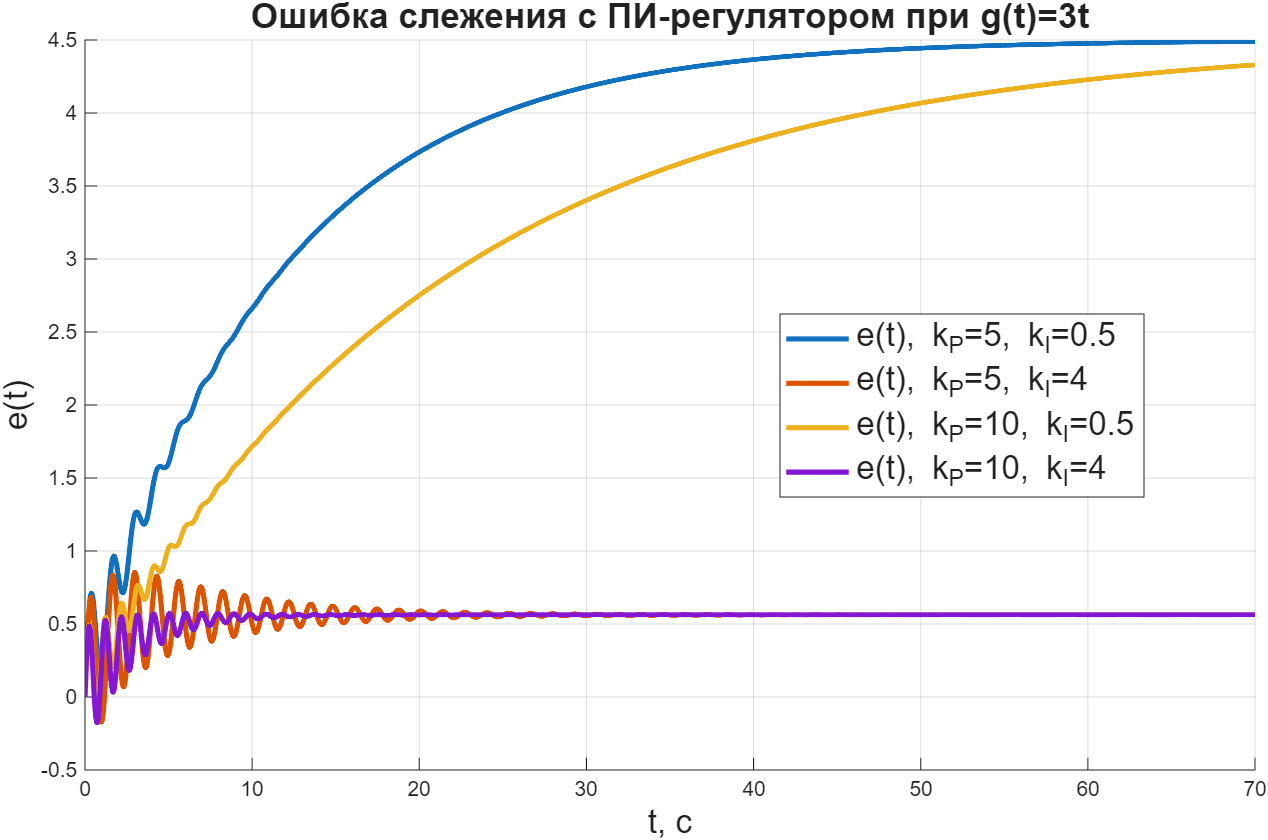
\includegraphics[width=0.75\linewidth]{images/Figure_4_5_2.png}
    \caption{Сопоставление ошибок системы при $g(t)=3t$}
    \label{fig:placeholder}
\end{figure}

\begin{figure}[H]
    \centering
    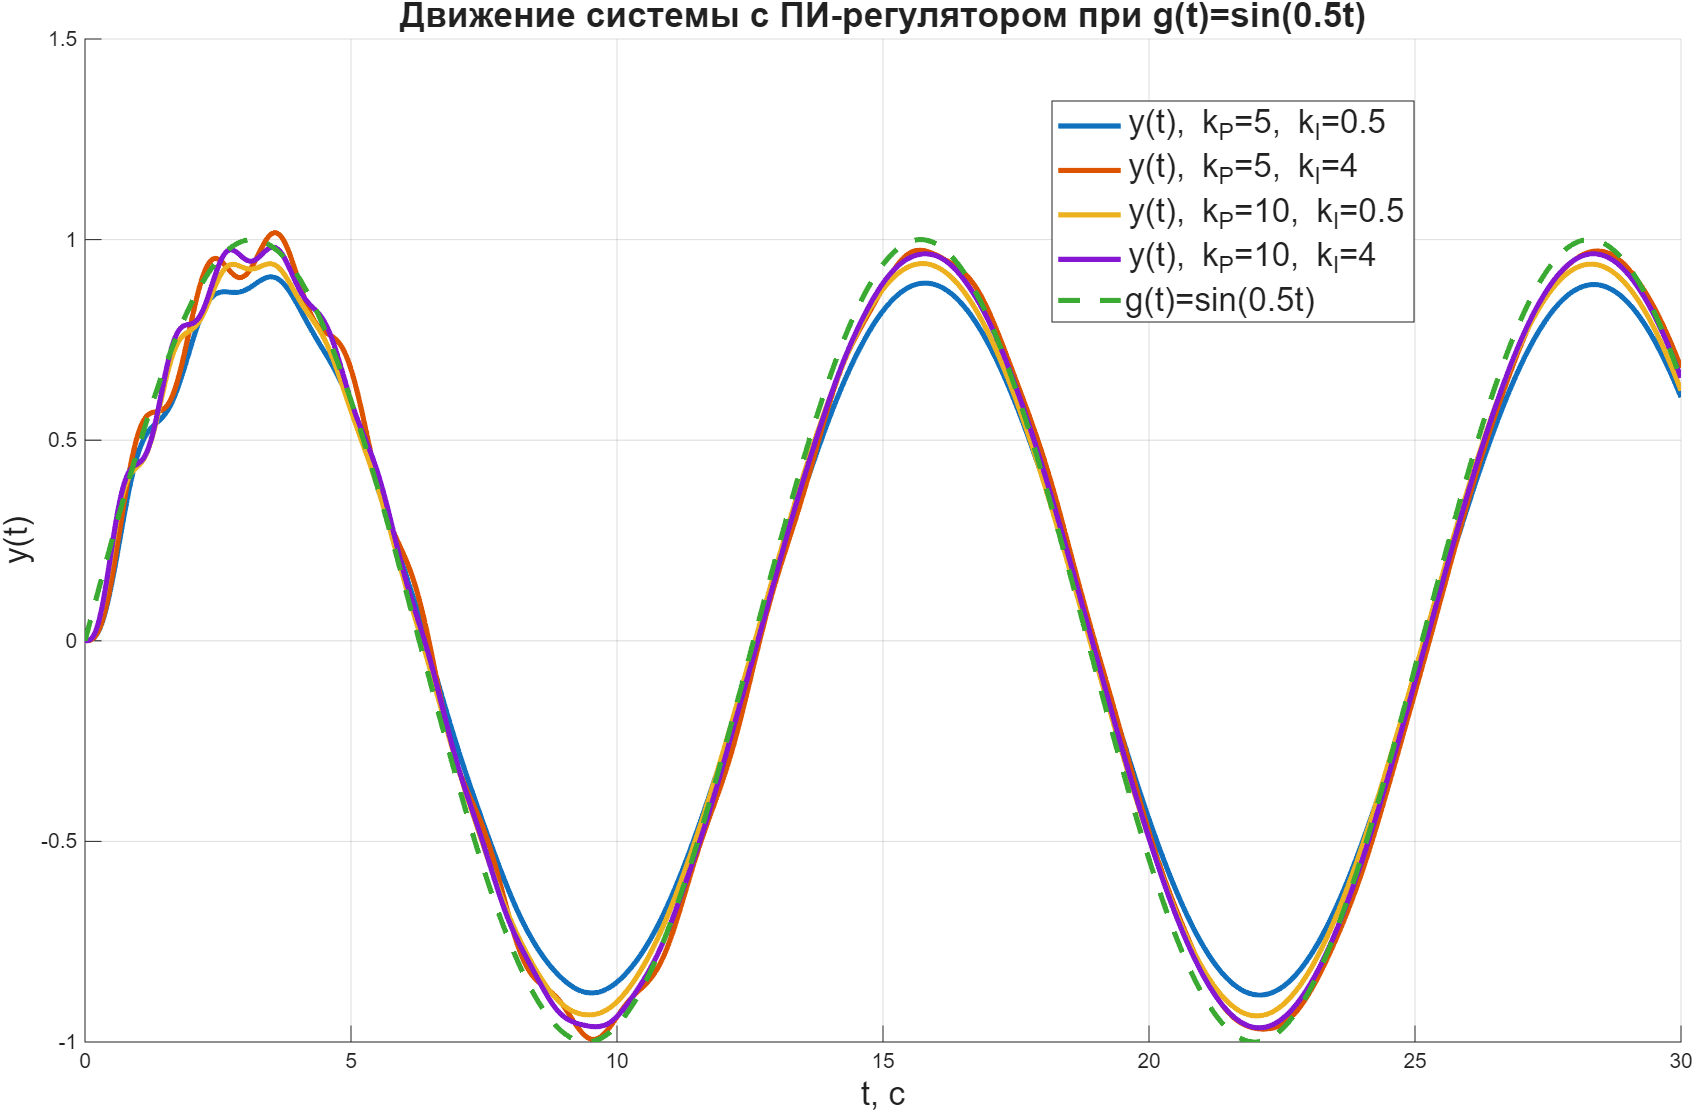
\includegraphics[width=0.75\linewidth]{images/Figure_4_5_3.png}
    \caption{Сопоставление движений системы при $g(t)=\sin(0.5t)$}
    \label{fig:placeholder}
\end{figure}

\begin{figure}[H]
    \centering
    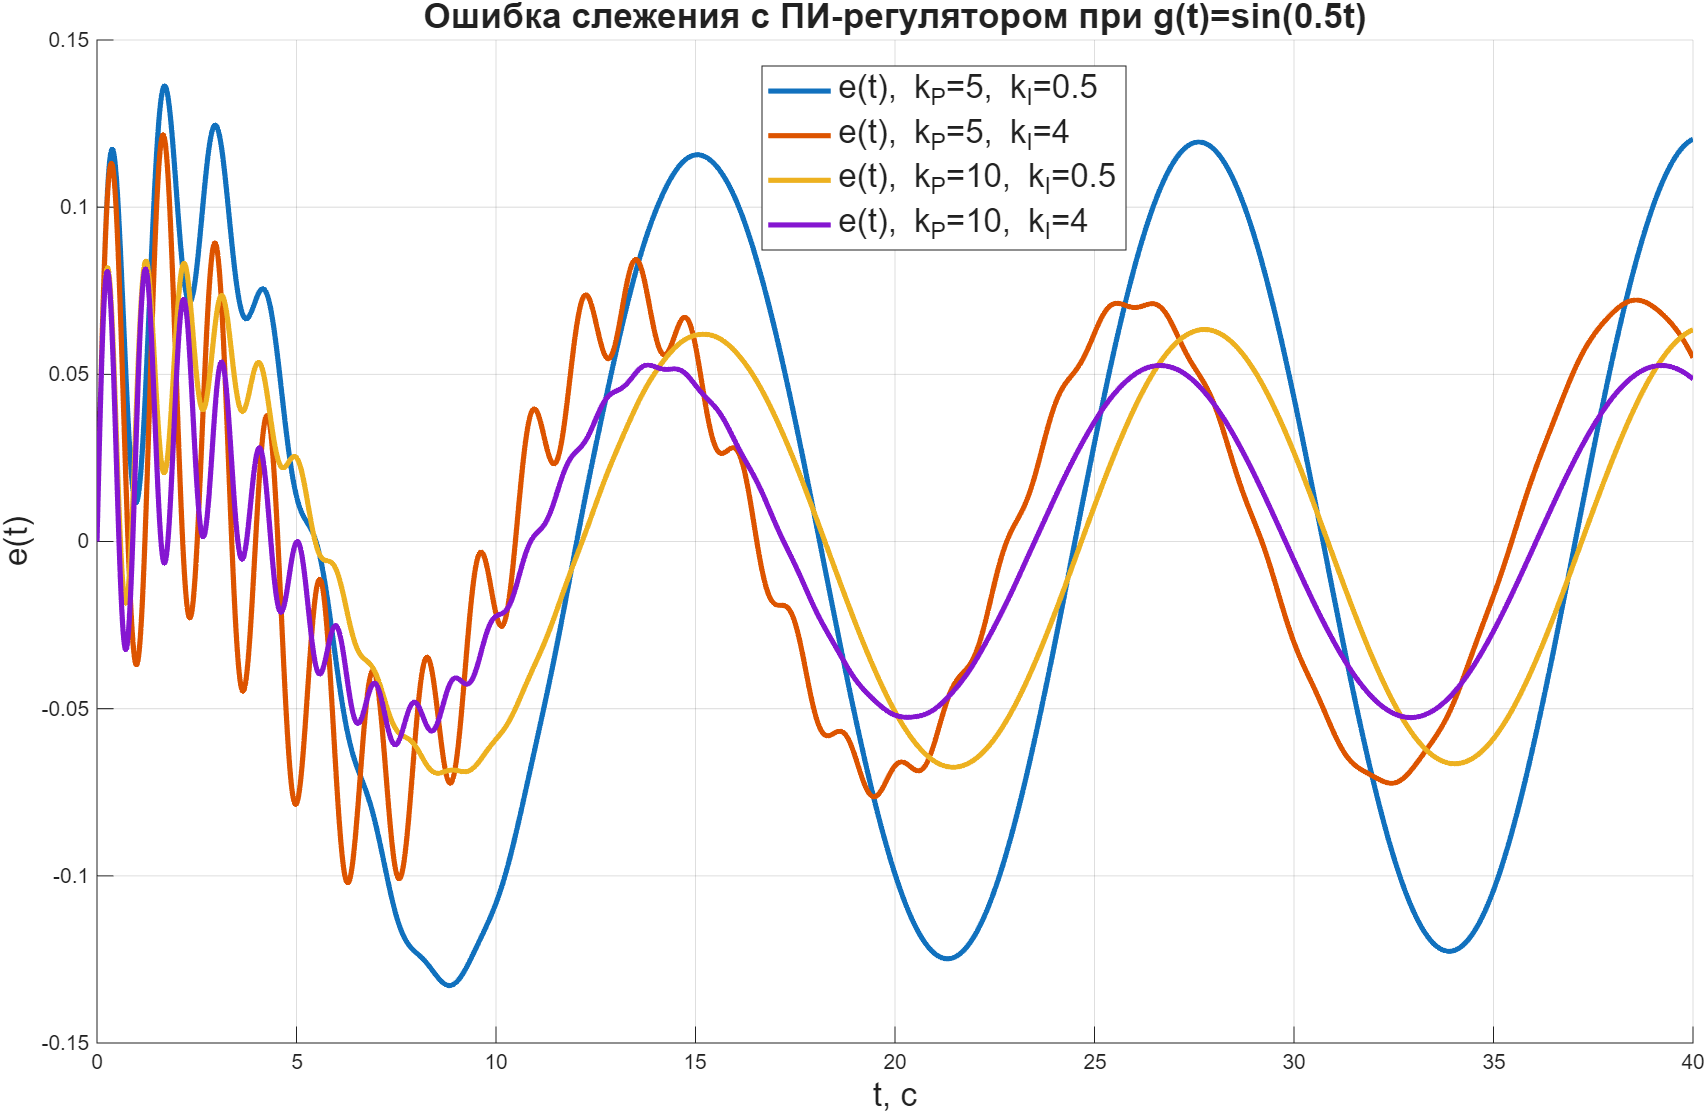
\includegraphics[width=0.75\linewidth]{images/Figure_4_5_4.png}
    \caption{Сопоставление ошибок системы при $g(t)=\sin(0.5t)$}
    \label{fig:placeholder}
\end{figure}

\subsection{Выводы}

В пятом задании была исследована система с пропорционально-интегральным
(ПИ) регулятором
\[
H(s)=\frac{k_{\text{И}}}{s}+k_{\text{П}}.
\]

В режиме движения с постоянной скоростью $g(t)=Vt$ установившаяся ошибка
определяется выражением
\[
e_{\text{уст}} = \frac{9}{4k_{\text{И}}},
\]
то есть зависит только от интегральной составляющей регулятора.
Увеличение $k_{\text{И}}$ приводит к уменьшению установившейся ошибки,
тогда как пропорциональная составляющая в основном влияет на
быстродействие и характер переходного процесса.

В режиме слежения за гармоническим сигналом $g(t)=A\sin(\omega t)$
система обеспечивает ограниченную периодическую ошибку.
Моделирование показало, что увеличение коэффициентов регулятора
уменьшает амплитуду ошибки и ускоряет переходный процесс,
однако полностью устранить ошибку для гармонического сигнала
ПИ-регулятор не позволяет.




\newpage

\section{Задание 6. Задача слежения за гармоническим сигналом (регулятор общего вида)}

\subsection{Исходные данные}

Рассмотрим замкнутую систему, заданную структурной схемой на рисунке \ref{fig:placeholder1}, где:

$$
H(s)=\dfrac{\sum \limits_{k=0}^{m}(b_ks^k)}{\sum \limits_{k=0}^{m}(a_ks^k)}
$$

Берем передаточную функцию в соответсвии с вариантом:

$$
W(s)=\dfrac{4}{s^2+s+3}
$$

Характеристики задающегося воздейстаия $g(t)$ также берем в соответсвии с вариантом:

\begin{table}[H]
    \centering
    \renewcommand{\arraystretch}{2} % увеличивает высоту строк
    \begin{tabular}{|c|c|c|c|}
    \hline
        $A$ & $Vt$ & $\dfrac{at^2}{2}$ & $A\sin(\omega t)$ \\[3pt] \hline
        $1$ & $3t$ & $0.5t^2$ & $\sin(0.5t)$ \\ \hline
    \end{tabular}
    \label{tab:placeholder}
\end{table}

\subsection{Аналитические расчеты}

Объект управления имеет придаточную функцию:

$$
W(s)=\dfrac{4}{s^2+s+3}.
$$

Задающее воздействие:

$$
g(t)=\sin(0.5t), \qquad \omega=0.5, \qquad G(s)=\dfrac{0.5}{s^2+0.25}
$$

Выберем порядок регулятора $m = 2$. Тогда регулятор примет вид:

$$
H(s)=\dfrac{b_2 s^2 + b_1 s + b_0}{s^2+0.25}
$$

Полином Баттерворта 4-го порядка:

$$
B_4(s)=s^4+2.6131\omega_0s^3+3.4142\omega_0^2s^2+2.6131\omega_0^3s+\omega_0^4
$$

Характеристическое уравнение замкнутой системы:

$$
(s^2+s+3)(s^2+0.25)+4(b_2 s^2 + b_1 s + b_0)=0
$$

$$
s^4+s^3+s^2(3.25+4b_2)+s(0.25+4b_1)+(0.75+4b_0)=0
$$

Возьмем $2.6131\omega_0=1$, тогда $\omega_0=0.383$

Тогда полином примет вид:

$$
B_4(s)=s^4+s^3+0.501s^2+0.147s+0.022
$$

Найдём коэффициенты b:

$$
\begin{cases}
    3.25+4b_2=0.501\\
    0.25+4b_1=0.147\\
    0.75+4b_0=0.022
\end{cases}
$$

$$
\begin{cases}
    b_2=-0.687\\
    b_1=-0.026\\
    b_0=-0.182
\end{cases}
$$

Тогда регулятор примет вид:

$$
H(s)=\dfrac{-0.687 s^2 -0.026 s -0.182}{s^2+0.25}
$$

Передаточная функция по ошибке имеет вид:

$$
W_e(s)=\dfrac{E(s)}{G(s)}=\dfrac{1}{1+W(s)H(s)}
$$

$$
W_e(s)=\dfrac{(s^2+s+3)(s^2+0.25)}{(s^2+s+3)(s^2+0.25)+4(-0.687s^2-0.026s-0.182)}
$$

Установившаяся ошибка:

$$
e_{\text{уст}}=\lim \limits_{t\to\infty}{e(t)}=\lim \limits_{s\to0}{sE(s)}=\lim \limits_{s\to0}{s\cdot W_e(s)\cdot G(s)}
$$

$$
e_{\text{уст}}=\lim \limits_{s\to0}{s\cdot \dfrac{(s^2+s+3)(s^2+0.25)}{(s^2+s+3)(s^2+0.25)+4(-0.687s^2-0.026s-0.182)}\cdot \dfrac{0.5}{s^2+0.25}}
$$

$$
e_{\text{уст}}=0
$$

\subsection{Структурные схемы}

\begin{figure}
    \centering
    \includegraphics[width=0.75\linewidth]{images/image_4_6_1.png}
    \caption{Структурная схема с регулятором общего вида}
    \label{fig:placeholder}
\end{figure}

\subsection{Графики сигналов $y(t)$, $e(t)$}

\begin{figure}[H]
    \centering
    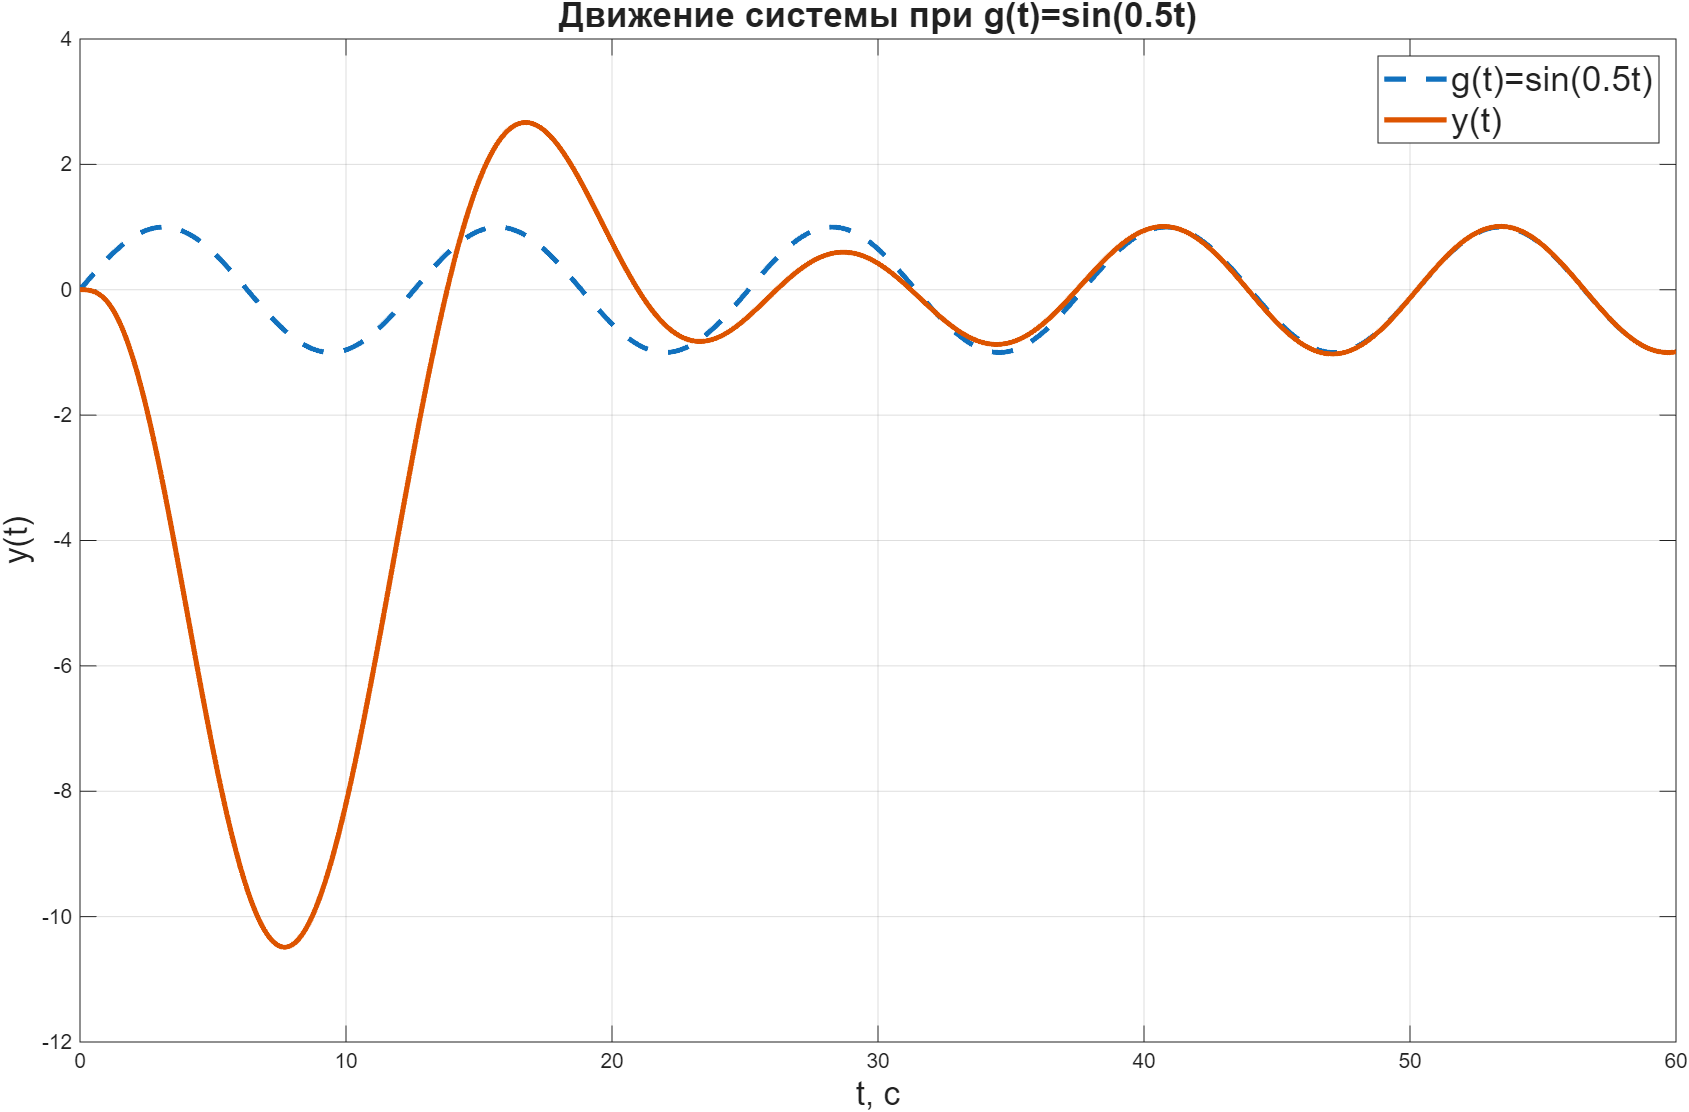
\includegraphics[width=0.75\linewidth]{images/Figure_4_6_1.png}
    \caption{График выхода замкнутой системы}
    \label{fig:placeholder}
\end{figure}

\begin{figure}[H]
    \centering
    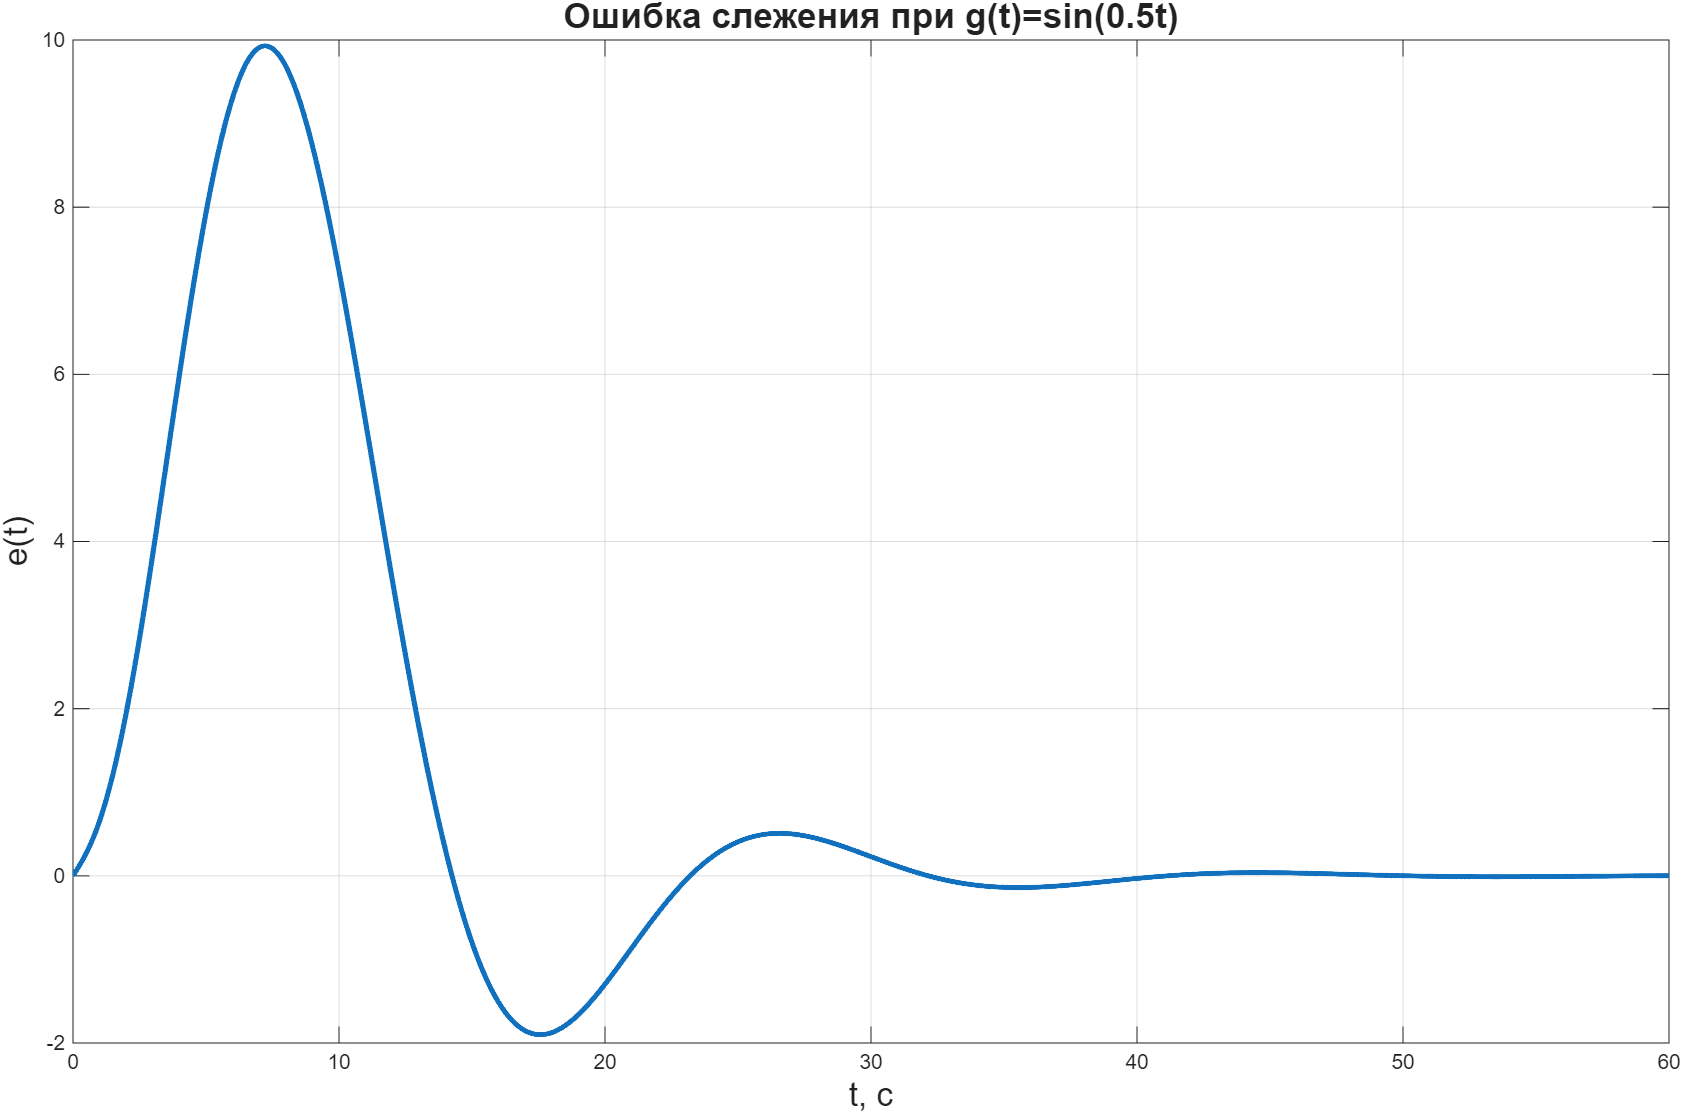
\includegraphics[width=0.75\linewidth]{images/Figure_4_6_2.png}
    \caption{График ошибки слежения}
    \label{fig:placeholder}
\end{figure}

Время по теореме подобия: $t_{\text{П}}^{'}=\dfrac{t_{\text{П}}}{\omega_0}$=$\dfrac{6.8}{0.383}=17.75$. Однако на практике, мы можем заметить, что время переходного процесса состовляет около 35 секунд. Следовательно, теоретическое время переходного процесса отличается от фактического.

\subsection{Выводы}

В шестом задании была рассмотрена задача синтеза физически реализуемого
регулятора общего вида
\[
H(s)=\frac{\sum_{k=0}^{m} b_k s^k}{\sum_{k=0}^{m} a_k s^k},
\]
обеспечивающего слежение за гармоническим сигналом
\[
g(t)=A\sin(\omega t)
\]
с нулевой установившейся ошибкой.

Нами был синтезирован регулятор общего вида, который обеспечивает нулевую установившуюся ошибку для нашей гармонической функции.

\section{Выводы}

В ходе выполнения лабораторной работы мы исследовали точностные свойства системы, астатизмы и регуляторы.

Мы увидели, что с помощью регуляторов можно стабилизировать изначально неустойчивую систему с помощью введения регуляторов. 

Экспериментально подтвердили связь между типом регулятора и порядком астатизма системы. Пропорциональный регулятор обеспечивает астатизм нулевого порядка, интегральный и пропорционально-интегральный
регуляторы обеспечивают астатизм первого порядка.

Синтезировали регулятор общего вида для обеспечения слежения за
гармоническими сигналами.
Показана необходимость компромисса между точностью, быстродействием и устойчивостью при выборе параметров регуляторов. 

Построили структурные схемы и провели моделирование в Matlab/Simulink.

\end{document}